%% !Mode:: "TeX:UTF-8"
\documentclass{mcmthesis}
%  \documentclass[CTeX = true]{mcmthesis}
\mcmsetup{tstyle=\color{red}\bfseries,%修改题号,队号的颜色和加粗显示,黑色可以修改为 black
        tcn = 2512625, problem = C, %修改队号,参赛题号
        sheet = true, titleinsheet = true, keywordsinsheet = true,
        titlepage = false, abstract = true}

% 代码块设置
    \usepackage{fontspec}
    \setmainfont{Charter} [
        Extension = .ttf,
        UprightFont = * Regular,
        BoldFont = * Bold, 
        ItalicFont = * Italic,
        BoldItalicFont = * Bold Italic
    ]
    \newfontfamily\consolasfont{Consola}[
        Extension = .ttf,
        UprightFont = *,
        BoldFont = *b,
        ItalicFont = *i,
        BoldItalicFont = *z
    ]

    \definecolor{bg}{rgb}{0.92,0.95,1.0} % Lighter blue fill
    \definecolor{borderblue}{rgb}{0.4,0.4,1.0} % Blue border
    \definecolor{commentcolor}{rgb}{0.4,0.85,0.4} % Softer green comment color

    \lstset{
        basicstyle=\consolasfont,  % Changed to use Consolas
        backgroundcolor=\color{bg},
        lineskip=1.5pt,
        frame=single,
        framesep=1mm,
        rulecolor=\color{borderblue}, % Blue border
        numbers=left,
        numberstyle=\small\color{gray}, % Changed from \tiny to \small
        keywordstyle=\color{blue},
        commentstyle=\color{green},
        commentstyle=\color{commentcolor}\itshape,
        stringstyle=\color{red},
        showstringspaces=false,
        breaklines=true,  % Ensure lines break within margins
        breakatwhitespace=true, % Allow breaking at whitespace
        prebreak=\raisebox{0ex}[0ex][0ex]{\ensuremath{\hookleftarrow}},
        postbreak=\raisebox{0ex}[0ex][0ex]{\ensuremath{\hookrightarrow}},
        escapeinside={(*@}{@*)},
        literate={-}{{\textendash}}1
    }
 
\usepackage{indentfirst}  %首行缩进,注释掉,首行就不再缩进。
\usepackage{lipsum}
\usepackage{wrapfig} % 图文绕排
\title{Mathematical Model for Prediction of Olympic Medal Counts}
\author{\small \href{https://www.latexstudio.net/}
  {\includegraphics[width=7cm]{mcmthesis-logo}}}
\date{\today}

\begin{document}
\begin{abstract}
    \par 
        SUMMARY HERE

\begin{keywords}
    keyword1; keyword2
\end{keywords}

\end{abstract}
\maketitle
\tableofcontents
\newpage

\section{Introduction}
\subsection{Problem Background}
The Olympic medal table is a key focus for nations and fans, reflecting athletic success and national pride. Predicting medal counts, however, is challenging due to the complex factors involved, such as event types, host country advantages, and the emergence of new competitors. This problem requires developing models exclusively based on the provided datasets, including historical medal tables, event breakdowns, and athlete performance.

Traditional forecasting methods, like OLS regression and Poisson models, struggle with accuracy, particularly for countries with zero or few medals. This problem emphasizes predicting medal breakthroughs for such nations, which demands innovative approaches beyond historical trends.

Key aspects include:
\begin{enumerate}
    \item Exploring the relationship between events and medal distributions.
    \item Examining host country advantages and their influence on results.
    \item Assessing the impact of "great coaches" on medal performance, identifying sports where targeted investment in coaching could make a difference.
    \item Projecting medal counts for the 2028 Los Angeles Olympics, including prediction intervals, while addressing uncertainty and potential breakthroughs for nations without prior Olympic success.
\end{enumerate}

\subsection{Literature Review}

Predicting Olympic medal counts has been a topic of interest for researchers across various fields, including economics, sociology, and sports science. Early studies, such as those by Ball (1972) and Grimes et al. (1974), \cite{1} focused on identifying fundamental socioeconomic and demographic factors that influence a nation's medal count. These studies emphasized the importance of population size and economic resources in determining Olympic success. Subsequent research, including work by Bernard and Busse (2004) and Xun Bian (2005) \cite{2}, further explored the impact of political systems and hosting advantages on medal counts, finding that hosting the Games and having a centrally-planned economy can significantly enhance a country's performance.

Recent advancements in statistical and machine learning techniques have led to more sophisticated models for predicting Olympic medals. Schlembach et al. (2022) \cite{5} applied a two-staged Random Forest model, incorporating a wide range of socioeconomic variables, including GDP, population, and public health indicators. This approach outperformed traditional models and naïve forecasts, demonstrating the potential of machine learning to improve prediction accuracy. Similarly, Forrest et al. (2010) \cite{4} enhanced traditional regression-based models by including additional regressors such as public spending on recreation and the effects of future hosts. These studies highlight the importance of considering multiple factors, including public health crises like COVID-19, in predicting Olympic performance.

Despite significant progress, predicting Olympic medals remains a complex task due to the interplay of numerous factors. It's recommended that future research should focus on incorporating more granular data, such as individual athlete performance and training conditions, to enhance prediction accuracy. Additionally, the use of panel data and advanced machine learning techniques, such as neural networks and ensemble methods, could provide further insights into the determinants of Olympic success. It's also deemed important to address the exogeneity of the total number of medals available and considering cultural factors, such as political freedom and gender equality. Overall, the field has evolved from simple correlation-based models to sophisticated machine learning algorithms, with traditional socioeconomic factors remaining significant predictors of Olympic success.

\subsection{Our Work}

Due to the limitation of usable dataset, we cannot explore many of the aforementioned factors in detail. Instead, we focus on developing a model that predicts Olympic medal counts based on historical data and sport-specific information. Our model has the following features:

\begin{enumerate}
    \item A two-stage model that first predicts the number of medals won by each country in each sport, then aggregates these predictions to estimate the total medal count.
    \item Trains and evaluates multiple models with different underlying algorithms on the same dataset, and use the best-performing model for prediction.
    \item Separates different countries into multiple clusters based on their historical medal counts (in which their comprehensive national power is also embodied \cite{7}), allowing for more accurate predictions for countries with similar overall strengths.
    \item A sensitivity analysis that assesses the impact of different factors on medal counts and identifies key drivers of success. 
\end{enumerate}

\section{Assumptions and Justifications} 

\begin{enumerate}
    \item \textbf{Homogeneity of Athletes}: We assume that athletes within the same country are homogeneous in terms of training, resources, and performance. This assumption simplifies the model by treating all athletes from a country as a single entity, ignoring individual variations.
    \item \textbf{Event Independence}: We assume that the outcomes of different events are independent of each other. This assumption allows us to model each event separately without considering potential correlations between them.
    \item \textbf{Historical Consistency}: We assume that historical trends in medal counts are consistent with future performance. This assumption underlies our prediction model, which relies on past data to forecast future outcomes.
    \item \textbf{Host Country Advantage}: We assume that host countries have a competitive advantage due to factors such as home crowd support and familiarity with the venues. This assumption is supported by previous research on the impact of hosting the Olympics on medal counts.
    
\end{enumerate}

\section{Notations and Definitions}


\section{Data Preprocessing}
% remember to mention some details
% 1. event/sport name changed over the course of time
% 2. some special years like 1906, when an unofficial Olympic Games was held. We need to exclude this year from our analysis.
% 3. event name ambiguity, e.g. 500+ events named "Men" and "Women"
\subsection{Early Attempts: Athlete-based Prediction}
First, we ruled out the approach of predicting medal counts based solely on the historical total medal data of countries, as this method is both logically flawed and overly simplistic. Given that the most detailed dataset provided includes information on individual Olympic competitors, their respective sports, events, and results, it is a natural and more precise approach to base medal predictions on the performance of individual athletes participating in specific events.

To facilitate this, we introduced a new column named "ID", which concatenates the athlete's name and event using an underscore ("\_"). This categorization enables us to construct a time series of medal data for each athlete and event, providing a robust foundation for applying predictive methods to estimate medal counts in future Olympics.

To put it lucidly, we added a column named "ID" which concatenated Name and Event with a "\_", which categorized the data in every individual and event. Then it's easier to create a time series of medal data out of it and apply certain method to predict the medal counts in the next Olympics.

Furthermore, we aimed to incorporate the host country as a training feature by matching it to competing country, while the dataset only provided host city. Recognizing the National Olympic Committee (NOC) code as a standardized and uniform identifier for countries, we created a dataset named "City\_NOC.csv" to serve as a dictionary containing all Olympic host cities and their corresponding NOC codes. Using this dictionary, we developed a Python script to add a new column, "host\_NOC", to the dataset while removing the original "City" column. Additionally, we excluded all data from the 1906 Olympics, as it was an informal event and disrupted the four-year cycle traditionally followed by the Olympic Games.

To further enhance data quality, we normalized medal counts by dividing them by their corresponding team sizes using a Python script. This normalization step ensured that the data accounted for the nature of team events, eliminating biases caused by repeated medal counts. We subsequently created a training dataset consisting of individual participants as rows and their corresponding medals earned and host NOC for each year as columns.

\subsection{Current Method: Sport/Event Oriented Data Preprocessing}

Despite these efforts, the athlete-based prediction results were significantly lower than the actual medal counts. This discrepancy likely stems from the instability of individual performances and the reality that most athletes do not participate in multiple Olympic Games, let alone win multiple medals. Consequently, we shifted to a more aggregated and macroscopic approach, categorizing data by country(NOC) and sport. We anticipated this method would yield more stable and reliable predictions.

To refine the dataset further, we addressed an issue where substitutes were included in the list of athletes, rendering team size unsuitable for normalizing medal counts. To resolve this, we removed columns such as Name, Sex, Team, and Event, which were irrelevant to the country- and sport-based approach. We then eliminated duplicate rows to create a cleaned dataset, "summerOly\_medal\_norepeat.csv", which contained all medals without repetition or omission.

Moreover, we recognized "No Medal" as a potential indicator of a country's capability in specific events. Countries participating in a sport are likely to perform better than those that do not. Therefore, we introduced a "No Medal" column as a parallel feature alongside the Gold, Silver, and Bronze medal counts for model training.

To enhance prediction accuracy, we planned to classify all participating countries into 5 tiers based on their historical medal counts. As a preparatory step, we preprocessed the data by summing historical medal counts from 2012 to 2024, which served as an indicator of a country's overall strength. Tier 5, the highest tier, comprised only the United States (USA) and China (CHN), which dominated in gold and total medal counts. Tier 4 and Tier 3 were identified based on a significant gap in gold medal counts, with Italy (38) marking the boundary between the two tiers and New Zealand (27) serving as the lower boundary of Tier 3. Tier 2 and Tier 1 were determined using total medal counts of 14 and 6, respectively. This tier-based categorization allowed for a more structured and nuanced analysis of countries' performance trends.

\subsection{Cumulative Medal-Winning Countries by Olympic Year}
Problem 1.2 requires projecting how many countries will earn their first medal in the next Olympics. To address this, we utilized the "summerOly\_medal\_norepeat.csv" dataset that was prepared earlier. A new column, "Medal", was added to the dataset, representing the sum of the "Gold", "Silver", and "Bronze" columns to indicate whether a given row corresponds to a medal-winning entry.

Subsequently, we developed a Python script to calculate the year in which each country earned its first medal. For countries that have not yet won any medals, the "Year" column was assigned the value 2028 to reflect the next Olympic cycle. Following this, another Python script was created to calculate the cumulative number of countries that had won medals up to each Olympic year. This cumulative count served as the foundational data for time series projection.

\section{Establishing the Model}

In this section, we outline the process of developing a regression-based model to predict medal counts (Gold, Silver and Bronze medals) for each country in the Los Angeles 2028 Summer Olympics. Our methodology accounts for historical performance, and hosting effects. The proposed approach includes estimates of uncertainty, prediction intervals, and measures of model performance. Additionally, we assess potential improvements or declines in medal counts for individual countries.

Thanks to the nature of this problem being inherently correlated to chronological projection and the provided data being complete with regard of countries, sports, events and individual athletes, we adopt time series analysis and regression models to predict medal counts for the 2028 Los Angeles Olympics.

To specify, we adopt a tier-based modeling strategy, aligning with the classification to be established in Task 1 - Subtask 3. Countries are grouped into five tiers based on their historical performance. Separate regression models are trained for each tier to capture the unique dynamics of countries within the same tier. The methodology involves the following steps:

\subsection{Data Loading \& Transformation}

\begin{itemize}
    \item \textbf{Loading:} We use data from the most recent eight Olympic Games, including information on hosting nations and medal counts (Gold, Silver, and Bronze) for each participating country.
    \item \textbf{Transformation:} Hosting nation information is one-hot encoded to introduce categorical variables. To address class imbalance, the SMOTE (Synthetic Minority Oversampling Technique) algorithm is applied, generating synthetic samples for underrepresented classes and balancing the dataset.
\end{itemize}

\begin{wrapfigure}{r}{8cm}  %这是图文混排的环境
    \centering
    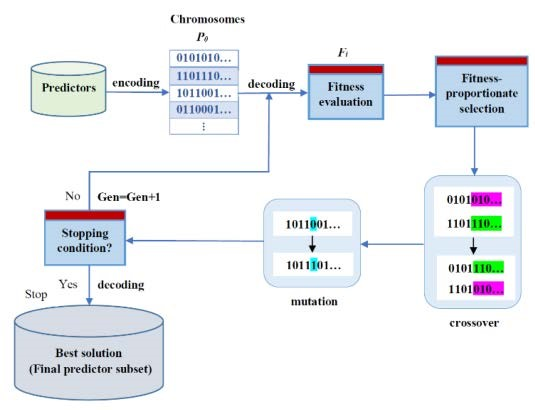
\includegraphics[width=0.9\linewidth,height=6cm]{pics/Multi-Agent_Optimization_Algorithm.jpg}
    \caption{mechanism of metaheuristic algorithm}
    \label{fig:metaheuristic_algorithm}
\end{wrapfigure}

\subsection{Feature Engineering}

Features are selected and optimized using metaheuristic algorithm to determine the most effective combinations. Like the image showed, this process involves transforming the feature selection problem into a binary optimization problem, where:
\begin{itemize}
    \item A value of 0 indicates the exclusion of a feature.
    \item A value of 1 indicates the inclusion of a feature.
\end{itemize}
A random forest model is trained iteratively with different feature combinations, and the performance of each combination is evaluated. Among all algorithms tested, the Sparrow Search Algorithm (SSA) achieved the best results for feature selection in Tier 1 Gold medal prediction.


\subsection{Data Splitting}

Given the relatively small dataset size, we adopt k-fold cross-validation to split the data into training, validation, and testing subsets. This approach ensures that the model is evaluated robustly across multiple splits of the data.

\subsection{Model Training}

We train several regression models on the training set, including:
\begin{itemize}
    \item LSBoost
    \item XGBoost
    \item Multivariate Linear Regression
    \item Gaussian Regression
    \item Decision Tree
    \item Random Forest
\end{itemize}

Each model is trained using the training set and evaluated on the validation set to determine the optimal hyperparameters.

\subsection{Model Evaluation}

The performance of each model is assessed on the test set using the following metrics:
\begin{itemize}
    \item Mean Absolute Error (MAE)
    \item Mean Absolute Percentage Error (MAPE)
    \item Mean Squared Error (MSE)
    \item Root Mean Squared Error (RMSE)
    \item Coefficient of Determination ($R^2$)
\end{itemize}

The evaluation result is stated as below. From the result we can see that each medal type can have very different best models. This phenomenon also vouches for the veracity of our tier-based modeling strategy.

\begin{lstlisting}
    RandomForest - Bronze:
    Prediction range: 2.14 to 7.84
    Mean prediction: 4.43
    Actual range: 2.00 to 9.00
    Actual mean: 4.29
    MSE: 11.1018
    MAE: 2.4743
    95% Prediction Interval: ±6.52
    
    GradientBoosting - Silver:
    Prediction range: 0.96 to 7.34
    Mean prediction: 4.39
    Actual range: 0.00 to 8.00
    Actual mean: 3.14
    MSE: 7.3283
    MAE: 2.0619
    95% Prediction Interval: ±4.71
    
    XGBoost - Gold:
    Prediction range: 1.01 to 6.13
    Mean prediction: 3.15
    Actual range: 0.00 to 4.00
    Actual mean: 2.86
    MSE: 3.4256
    MAE: 1.6301
    95% Prediction Interval: ±3.58
    
    Best model for Bronze (MAE=2.4743): RandomForest
    Best model for Silver (MAE=2.0619): GradientBoosting
    Best model for Gold (MAE=1.6301): XGBoost
\end{lstlisting}
    

\subsection{Model Selection}

The best-performing model is selected using the TOPSIS (Technique for Order Preference by Similarity to Ideal Solution) method. This approach ensures a balanced evaluation by simultaneously considering models with:
\begin{itemize}
    \item Smaller values of MAE, MAPE, MSE, and RMSE.
    \item Larger values of $R^2$ (closer to 1 indicates better fit).
\end{itemize}
In the Tier 1 Gold medal prediction model, XGBoost exhibited the best performance after evaluation.

\subsection{Model Optimization}

We apply various optimization algorithms to enhance model performance further. The algorithms tested include:
SSA \cite{8}, DBO \cite{9}, SCA \cite{10}, SA \cite{11}, PSO \cite{12}, SO \cite{13}, POA \cite{14},  
GWO \cite{15}, IGWO \cite{16}, AVOA \cite{17}.

As an example, SSA algorithm demonstrated the best results for optimizing the Tier 1 Gold medal prediction model, and the following figure shows the optimization outcome.

\begin{figure}[htbp]
    \centering
    % First row
    \begin{minipage}[t]{0.3\textwidth}
        \centering
        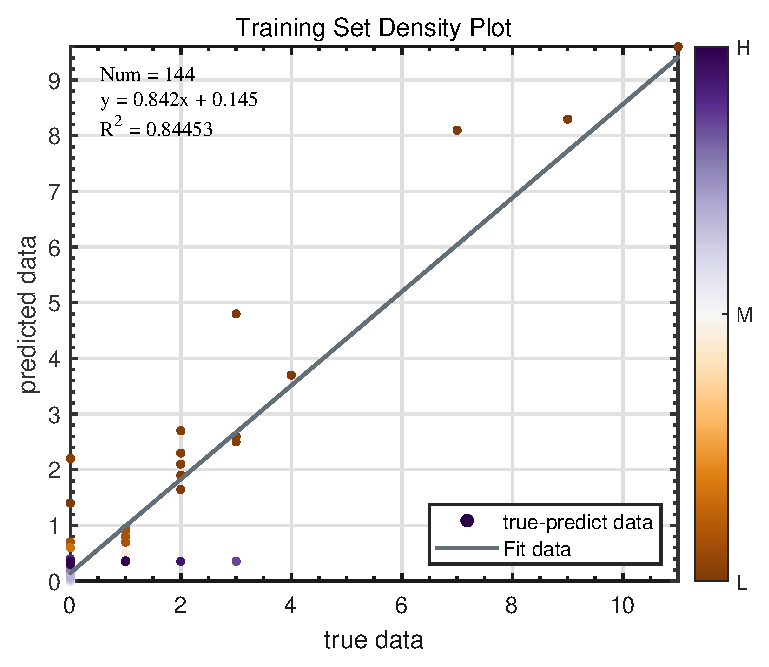
\includegraphics[width=2.2in, keepaspectratio]{pics/1.eps}
        \label{fig:image1}
    \end{minipage}
    \hfill
    \begin{minipage}[t]{0.3\textwidth}
        \centering
        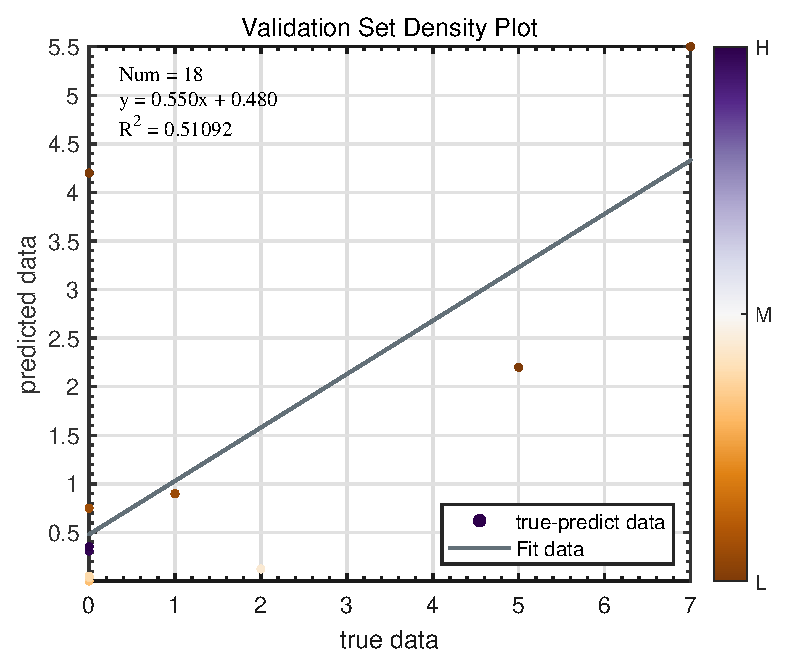
\includegraphics[width=2.2in, keepaspectratio]{pics/3.eps}
        \label{fig:image2}
    \end{minipage}
    \hfill
    \begin{minipage}[t]{0.3\textwidth}
        \centering
        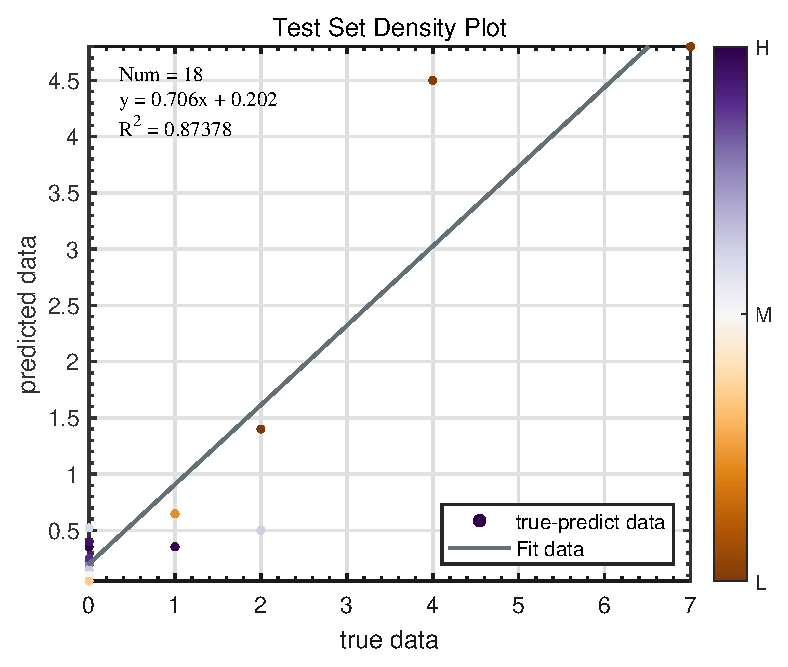
\includegraphics[width=2.2in, keepaspectratio]{pics/5.eps}
        \label{fig:image3}
    \end{minipage}
    
    \vspace{0.4cm} % Space between rows
    
    % Second row
    \begin{minipage}[t]{0.3\textwidth}
        \centering
        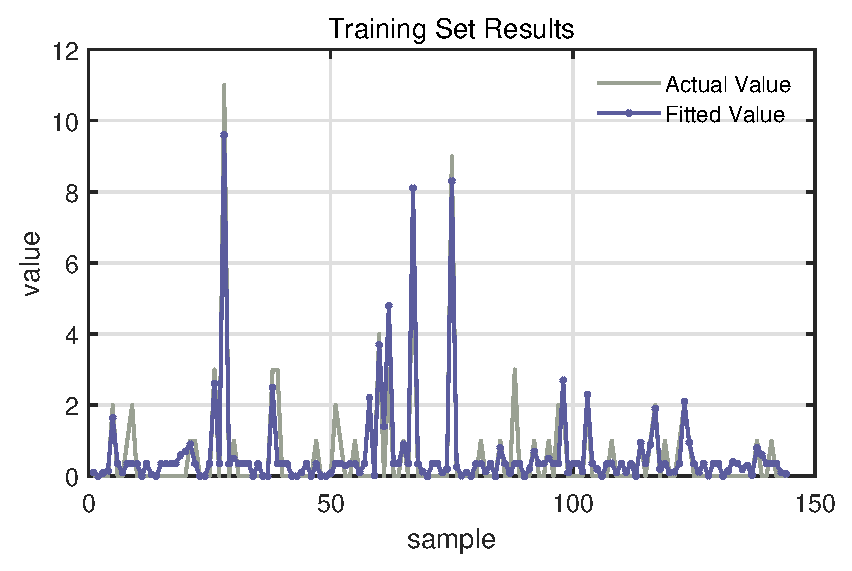
\includegraphics[width=2.2in, keepaspectratio]{pics/2.eps}
        \label{fig:image4}
    \end{minipage}
    \hfill
    \begin{minipage}[t]{0.3\textwidth}
        \centering
        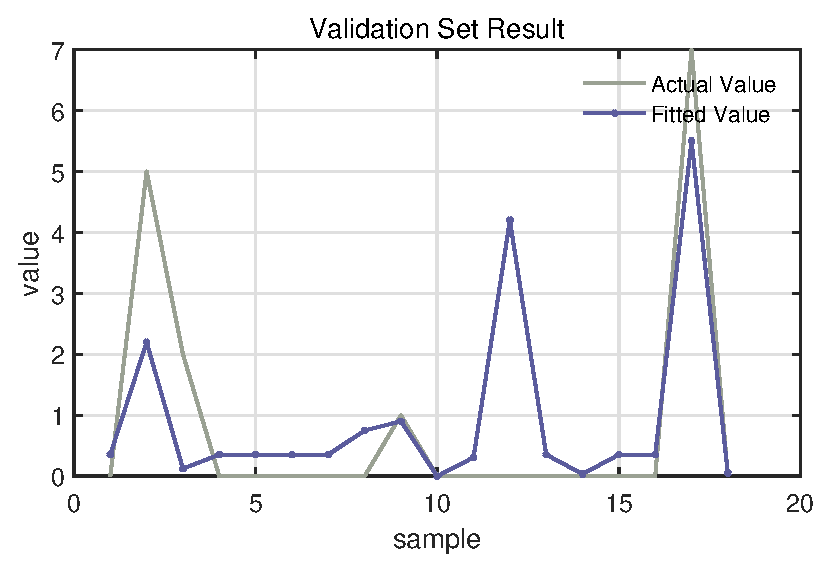
\includegraphics[width=2.2in, keepaspectratio]{pics/4.eps}
        \label{fig:image5}
    \end{minipage}
    \hfill
    \begin{minipage}[t]{0.3\textwidth}
        \centering
        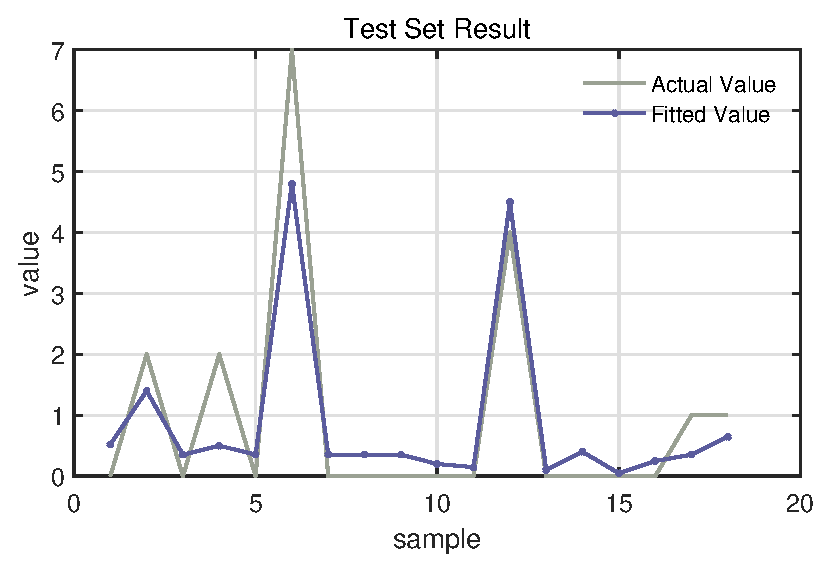
\includegraphics[width=2.2in, keepaspectratio]{pics/6.eps}
        \label{fig:image6}
    \end{minipage}
    
    \caption{Six smaller EPS images arranged in two rows and three columns, resized to fit the page.}
    \label{fig:smaller_eps_images}
\end{figure}


    

\subsection{Uncertainty Quantification and Prediction Intervals}

To quantify the uncertainty in model predictions, we use Gaussian Probability Interval Prediction. This method calculates prediction intervals, providing upper and lower bounds for the estimated medal counts. The intervals represent the range within which the actual medal counts are expected to fall with a specified confidence level.
\begin{figure}[htbp]
    \centering
    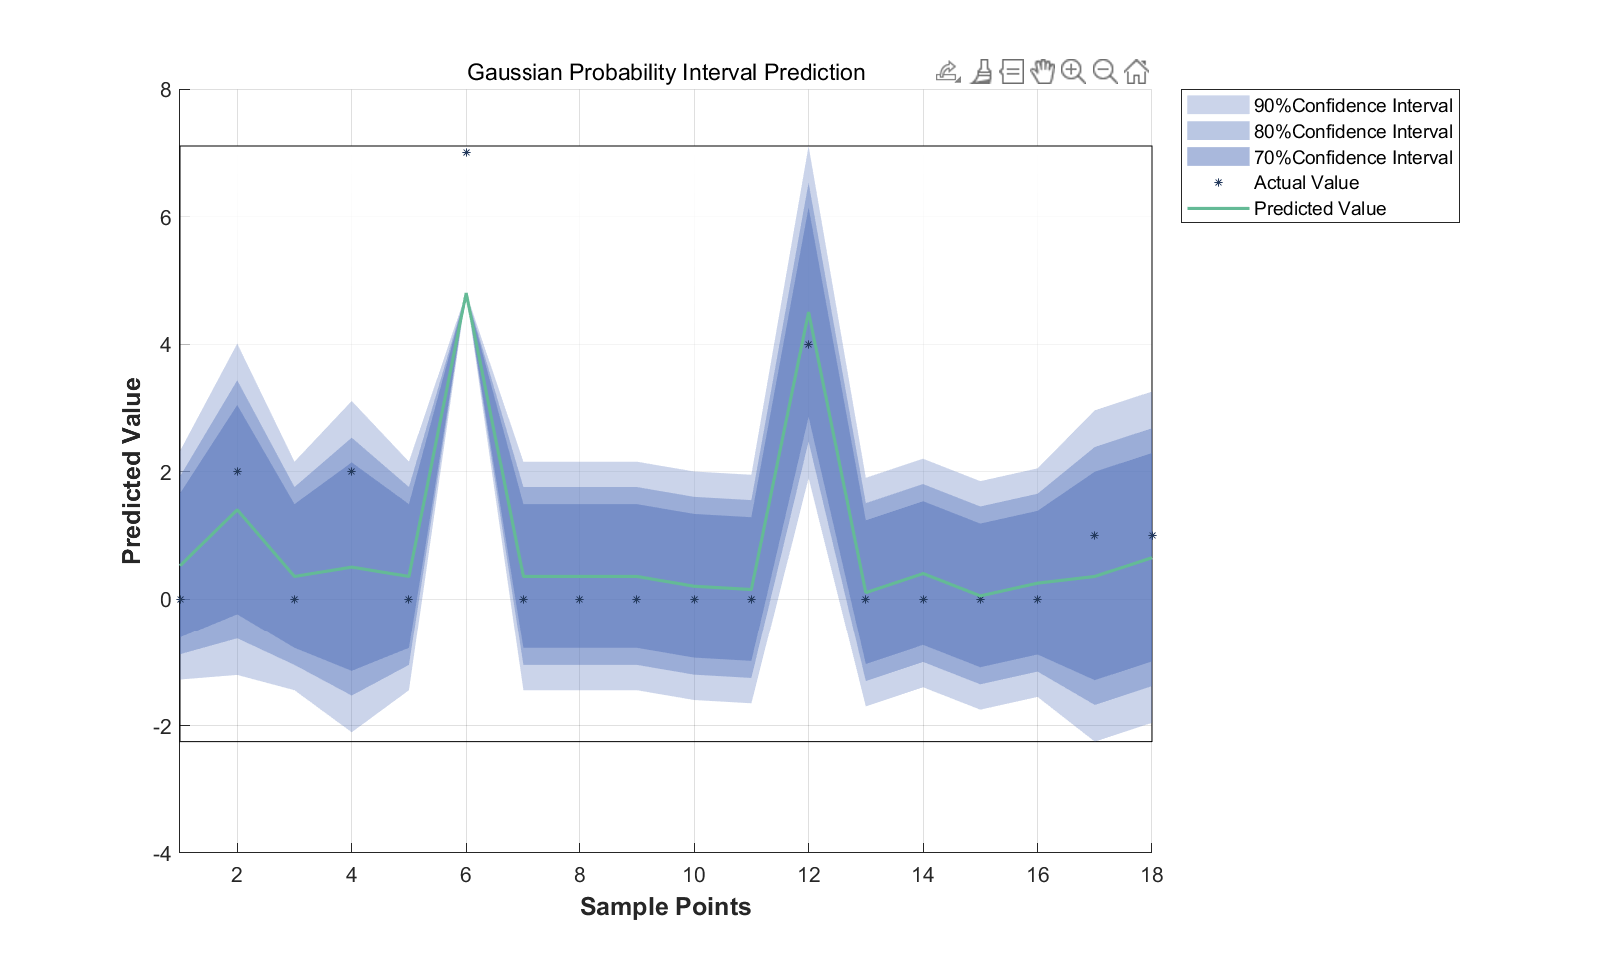
\includegraphics[width=3.33in, keepaspectratio]{pics/Gaussian Probability Interval Prediction.eps}  
\end{figure}

\subsection{Conclusion}

The tier-based regression modeling approach provides a structured and efficient framework for predicting Olympic medal counts. By incorporating historical performance, host nation effects, and optimization techniques, the model achieves robust performance and reliable projections. The results offer actionable insights for countries aiming to improve their Olympic performance.

\section{Task1 --- Employing the model for prediction}

\subsection{Subtask 1 --- Predicting Medal Counts for the 2028 Los Angeles Olympics}

\subsubsection{Prediction Results}
We tested the established model to predict medal counts for the 2028 Los Angeles Olympics. The resulting medal table is as follows: (results rounded to one decimal place, and the prediction intervals attached are calculated at a 95\% confidence level)

\begin{table}[htbp]
    \centering
    \begin{tabular}{|c|c|c|c|c|c|c|c|c|c|c|}
        \hline
        NOC & B & S & G & BL & BU & SL & SU & GL & GU & Tot \\
        \hline
        USA & 48.8 & 45.3 & 45.9 & 46.3 & 51.3 & 43.9 & 46.8 & 43.3 & 48.6 & 140.1 \\
        CHN & 27.3 & 30.1 & 46.7 & 25 & 29.6 & 28.8 & 31.4 & 44.3 & 49.1 & 104.1 \\
        GBR & 38.8 & 24.6 & 20.5 & 36.5 & 41.1 & 23.3 & 25.9 & 18.1 & 22.9 & 83.9 \\
        JPN & 19.1 & 22 & 26.3 & 16.8 & 21.4 & 20.7 & 23.3 & 23.9 & 28.7 & 67.4 \\
        FRA & 30.4 & 12.1 & 21.3 & 28.1 & 32.7 & 10.8 & 13.4 & 18.9 & 23.7 & 63.8 \\
        AUS & 18.3 & 15.4 & 21.7 & 16 & 20.6 & 14.1 & 16.7 & 19.3 & 24.1 & 55.4 \\
        ITA & 15.4 & 11.5 & 13.6 & 13.1 & 17.7 & 10.2 & 12.9 & 11.2 & 16 & 40.6 \\
        NED & 17 & 10.1 & 11.7 & 14.7 & 19.3 & 8.8 & 11.4 & 9.3 & 14.1 & 38.9 \\
        GER & 6.4 & 18 & 10.8 & 4.1 & 8.7 & 16.6 & 19.3 & 8.4 & 13.2 & 35.2 \\
        CAN & 11.5 & 5.5 & 10.5 & 9.2 & 13.7 & 4.2 & 6.8 & 8.1 & 12.9 & 27.4 \\
        KOR & 10.7 & 7.9 & 7.8 & 8.4 & 13 & 6.6 & 9.2 & 5.4 & 10.2 & 26.4 \\
        BRA & 5.6 & 8.2 & 6.8 & 3.3 & 7.9 & 6.9 & 9.5 & 4.4 & 9.2 & 20.6 \\
        NZL & 1.7 & 5.5 & 12.5 & 0 & 4 & 4.2 & 6.8 & 10.1 & 14.9 & 19.8 \\
        UKR & 7.9 & 5.2 & 5.7 & 5.6 & 10.2 & 3.9 & 6.5 & 3.3 & 8.1 & 18.8 \\
        ESP & 7.5 & 5.7 & 2.6 & 5.2 & 9.8 & 4.4 & 7 & 0.2 & 5 & 15.8 \\
        HUN & 3.9 & 7.5 & 3 & 1.6 & 6.2 & 6.2 & 8.8 & 0.6 & 5.4 & 14.3 \\
        AZE & 5 & 5.2 & 3 & 2.7 & 7.3 & 3.9 & 6.5 & 0.6 & 5.4 & 13.2 \\
        DEN & 6.6 & 3.8 & 2.3 & 4.3 & 8.9 & 2.5 & 5.1 & 0 & 4.8 & 12.7 \\
        BEL & 5.5 & 2 & 5.2 & 3.2 & 7.8 & 0.7 & 3.3 & 2.8 & 7.6 & 12.7 \\
        IRI & 4.9 & 3.1 & 3.5 & 2.6 & 7.2 & 1.8 & 4.4 & 1.1 & 5.9 & 11.5 \\
        JAM & 2.5 & 6.6 & 2.3 & 0.2 & 4.8 & 5.3 & 7.9 & 0 & 4.7 & 11.4 \\
        KAZ & 4.6 & 3.8 & 2.8 & 2.3 & 6.9 & 2.5 & 5.2 & 0.4 & 5.2 & 11.3 \\
        CUB & 5.7 & 3.2 & 2.1 & 3.4 & 8 & 1.9 & 4.5 & 0 & 4.5 & 11.1 \\
        KEN & 3.2 & 5.4 & 2.4 & 0.9 & 5.5 & 4 & 6.7 & 0 & 4.8 & 11 \\
        SWE & 3.2 & 3.6 & 3.9 & 0.9 & 5.5 & 2.3 & 4.9 & 1.5 & 6.3 & 10.7 \\
        SUI & 5.7 & 2.5 & 2.4 & 3.4 & 8 & 1.2 & 3.8 & 0 & 4.8 & 10.6 \\
        POL & 4.6 & 2.2 & 3.2 & 2.3 & 6.9 & 0.9 & 3.5 & 0.8 & 5.6 & 9.9 \\
        GRE & 6.8 & 1.2 & 0.7 & 4.5 & 9.1 & 0 & 2.6 & 0 & 3.1 & 8.7 \\
        UZB & 3.2 & 3.1 & 2.4 & 0.9 & 5.5 & 1.8 & 4.4 & 0 & 4.8 & 8.7 \\
        GEO & 3.2 & 2.4 & 2.7 & 0.9 & 5.5 & 1.1 & 3.8 & 0.3 & 5.1 & 8.4 \\
        LTU & 3.2 & 1.6 & 2.5 & 0.9 & 5.5 & 0.3 & 2.9 & 0.1 & 4.9 & 7.3 \\
        CRO & 3.1 & 3.2 & 0.9 & 0.8 & 5.4 & 1.9 & 4.5 & 0 & 3.3 & 7.3 \\
        TUR & 4.8 & 2.6 & 0 & 2.5 & 7.1 & 1.3 & 3.9 & 0 & 2.1 & 7.1 \\
        ROU & 3.3 & 0.9 & 2.9 & 1 & 5.6 & 0 & 2.2 & 0.5 & 5.3 & 7.1 \\
        BUL & 2.5 & 1.4 & 3 & 0.2 & 4.8 & 0.1 & 2.7 & 0.6 & 5.4 & 6.9 \\
        NOR & 3.8 & 1.4 & 1.4 & 1.5 & 6.1 & 0.1 & 2.7 & 0 & 3.8 & 6.6 \\
        THA & 2.6 & 2.3 & 1.5 & 0.3 & 4.9 & 1 & 3.6 & 0 & 3.9 & 6.4 \\
        CZE & 2 & 2.7 & 1.4 & 0 & 4.2 & 1.4 & 4.1 & 0 & 3.8 & 6.1 \\
        RSA & 2.1 & 3.4 & 0.6 & 0 & 4.4 & 2 & 4.7 & 0 & 3 & 6.1 \\
        ETH & 1 & 2.8 & 1.2 & 0 & 3.3 & 1.5 & 4.1 & 0 & 3.6 & 5 \\
        TPE & 2.2 & 1.3 & 1.5 & 0 & 4.5 & 0 & 2.6 & 0 & 3.9 & 5 \\
        IND & 1.4 & 1.9 & 1.6 & 0 & 3.7 & 0.5 & 3.2 & 0 & 4 & 4.9 \\
        MEX & 2.2 & 2.7 & 0 & 0 & 4.5 & 1.4 & 4 & 0 & 2.2 & 4.8 \\
        ... & ... & ... & ... & ... & ... & ... & ... & ... & ... & ... \\
    \end{tabular}
    \caption{Predicted medal counts for 2028 Los Angeles Olympics. B: Bronze, S: Silver, G: Gold, BL: Bronze Lower Bound, BU: Bronze Upper Bound, SL: Silver Lower Bound, SU: Silver Upper Bound, GL: Gold Lower Bound, GU: Gold Upper Bound. Due to space constraints, only the top 43 countries are shown.}
    \label{tab:medal_counts}
\end{table}

\subsubsection{Analysis of Prediction Results}

In this section, we analyze the improvements or declines in medal counts. We define \textit{"improvement"} and \textit{"decline"} as follows in order to separate them from normal fluctuations:

\begin{itemize}
    \item \textbf{Improvement:} If the predicted medal count for a country in 2028 is higher than its medal count from the previous Olympics more than a constant \textit{X} percent (\textbf{Condition 1}) or for every type of medal, the count doesn't decrease and at least one type of medal shows increase in count (\textbf{Condition 2}), we consider it an improvement.
    \item \textbf{Decline:} If the predicted medal count for a country in 2028 is lower than its medal count from the previous Olympics more than a constant \textit{X} percent (\textbf{Condition 1}) or for every type of medal, the count doesn't increase and at least one type of medal shows decrease in count (\textbf{Condition 2}), we consider it a decline.
\end{itemize}

With \textit{X} set to 15\%, we identified the following countries that are expected to improve or decline in medal counts at the 2028 Los Angeles Olympics:

\begin{table}[htbp]
    \centering
    \begin{tabular}{|c|c|c|}
        \hline
        NOC & Change & Conditions Met \\
        \hline
        ARG & Imp & 1, 2 \\
        AZE & Imp & 1, 2 \\
        BEL & Imp & 1 \\
        CHN & Imp & 2 \\
        CUB & Imp & 1 \\
        DEN & Imp & 1, 2 \\
        ETH & Imp & 1 \\
        GBR & Imp & 1, 2 \\
        GEO & Imp & 1 \\
        INA & Imp & 1 \\
        JAM & Imp & 1, 2 \\
        JPN & Imp & 1, 2 \\
        KAZ & Imp & 1, 2 \\
        LTU & Imp & 1 \\
        SUI & Imp & 1, 2 \\
        SVK & Imp & 1 \\
        UKR & Imp & 1, 2 \\
        USA & Imp & 2 \\
        HUN & Dec & 1 \\
        IND & Dec & 1 \\
        KOR & Dec & 1 \\
        MAR & Dec & 1 \\
        NOR & Dec & 1 \\
        POR & Dec & 1 \\
        ROU & Dec & 1 \\
        TUR & Dec & 2 \\
        UZB & Dec & 1 \\
        \hline
    \end{tabular}
    \caption{Countries with Predicted Changes in Medal Counts for the 2028 Los Angeles Olympics}
    \label{tab:medal_changes}
\end{table}








\subsection{Subtask 2 --- Predicting the Number of Countries Winning Their First Medal}

In this subtask, we aim to predict the number of countries that will win their first Olympic medal at the 2028 Los Angeles Olympics. This involves analyzing historical data to identify trends and factors that contribute to countries winning their first medals and applying these insights to make predictions for the upcoming Olympics.

\subsubsection{Analysis}
Firstly, we calculated historical data on countries that have won their first Olympic medals in past Games, which is done in Data Preprocessing. The visualization of this dataset is shown below.

%! TODO: Fig. Cumulative Medal-Winning Countries by Olympic Year

\subsubsection{Results}

Based on our analysis and model predictions, we estimate that approximately $X$ countries will win their first Olympic medal at the 2028 Los Angeles Olympics. This prediction is based on the trends observed in historical data and the identified key features that contribute to a country's likelihood of winning its first medal.


\subsection{Subtask 3.1 --- Exploring the Relationship Between Event Count and Medal Count}

In this subtask, we investigate the relationship between the number and types of events a country participates in and the number of medals it earns. The analysis is performed using data from the 2024 Olympics, focusing on three primary aspects: visualization, correlation analysis, and interpretation of results.

\subsubsection{Visualization}
To better understand the relationship between event count and medal count, we employed two visualization methods:
\begin{itemize}
    \item \textbf{Scatter Plot}: A scatter plot was created to display the relationship between the number of events a country participates in (event count) and the number of medals it earns (medal count).  
    \item \textbf{Box Plot}: To further analyze the distribution of medal counts across different event count intervals, a box plot was used. This visualization captures the median, interquartile range (IQR), and outliers of medal counts for countries grouped into event count bins. The box plot reveals that countries with higher event participation tend to have a wider distribution of medal counts, suggesting greater variability.
\end{itemize}

    
\begin{figure}[htbp]
    \begin{minipage}[t]{0.5\textwidth}
        \centering
        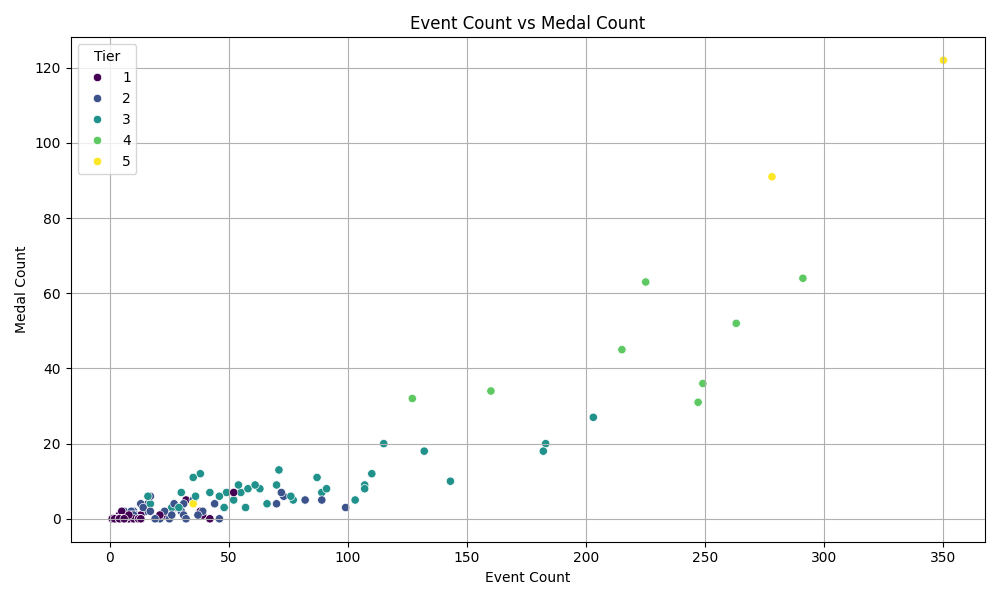
\includegraphics[width=0.8\textwidth]{pics/event_count_vs_medal_count.png}
    \end{minipage}
    \begin{minipage}[t]{0.5\textwidth}
        \centering
        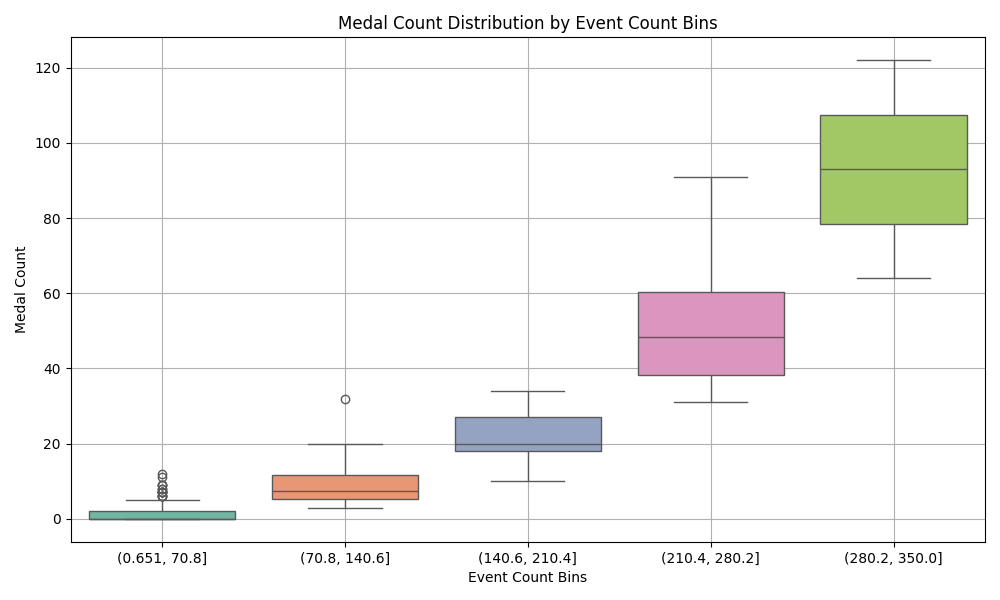
\includegraphics[width=0.9\textwidth]{pics/medal_count_distribution_by_event_count_bins.png}
    \end{minipage}
    \caption{Visualizations: (Left) Scatter plot showing the correlation; 
    (Right) Box plot depicting the distributions.}
\end{figure}

    To better understand the relationship between event count and medal count, countries were grouped into five distinct tiers based on their competitive performance using the K-means clustering algorithm. This method allowed for the segmentation of countries into groups with similar competition characteristics, providing a more nuanced analysis of the underlying relationships.

    The decision to use K-means clustering was motivated by the scatter plot observations, which suggested heterogeneous patterns in the event count and medal count relationship across different types of countries. The clustering process was informed by previous medal achievements(first gold medals, then total medals), ensuring that the grouping reflected meaningful competitive distinctions.
    
    Once the countries were assigned to tiers, we conducted separate correlation analyses within each tier. This approach allowed for a targeted examination of the relationship between event count and medal count, accounting for the differences in competitive capabilities and strategies across tiers. Spearman's correlation coefficient was used to measure the strength and direction of the relationship, as it is well-suited for non-parametric data and can handle potential non-linearities. The results are shown in following Table.


\begin{table}[h!]
    \centering
    \begin{tabular}{ccc}
    \toprule
    \textbf{Tier} & \textbf{Spearman Correlation} & \textbf{p-value} \\
    \midrule
    1 & 0.38 & $2.16 \times 10^{-5}$ \\
    2 & 0.39 & 0.01 \\
    3 & 0.61 & $4.99 \times 10^{-5}$ \\
    4 & 0.57 & 0.13 \\
    5 & 0.98 & 0.02 \\
    \bottomrule
    \end{tabular}
    \caption{Spearman correlation and p-values across different tiers.}
    \label{tab1}
\end{table}

\subsubsection{Interpretation of Results}
The analysis indicates that for most tiers (1, 2, 4, and 5), there is a statistically significant positive relationship between event count and medal count ($p < 0.05$). This suggests that the number of events a country participates in positively impacts its medal count. For Tier 3, the $p$-value is greater than 0.05, indicating no statistically significant correlation between event count and medal count within this group. This anomaly could be due to specific factors such as high variability in event outcomes or unmeasured country-specific attributes.

The correlation coefficients also show a general trend where the relationship between event count and medal count strengthens as the tier increases. This aligns with the expectation that more competitive countries (higher tiers) are better equipped to convert event participation into medals due to superior resources, training, and athletes.

\subsubsection{Conclusions and Recommendations(Optional)}
The results of this analysis demonstrate the critical importance of event participation in achieving higher medal counts. Based on these findings, we propose the following recommendations for countries aiming to improve their medal counts in the 2028 Los Angeles Olympics:
\begin{itemize}
    \item \textbf{Strategic Participation}: Countries should carefully select events where they have a competitive advantage and allocate resources to maximize medal potential.
    \item \textbf{Investment in Training and Resources}: Especially for lower-tier countries, investing in infrastructure, coaching, and athlete preparation can increase their ability to perform well across a broader range of events.
    \item \textbf{Focus on Key Events}: Higher-tier countries should focus on optimizing performance in key events where they historically perform well, while also expanding into new events with medal potential.
\end{itemize}
This analysis underscores the interplay between event participation and medal success, offering actionable insights for Olympic planning and preparation.

\subsection{Subtask 3.2 --- Identifying the Most Important Sports for Various Countries}

This subtask aims to determine the most significant sports for different countries based on their historical performance in the Olympics. To achieve this, we develop a method to calculate the importance of each event and sport, both at the country level and globally. 

\subsubsection{Notations and Definitions}
Let us define the following notations for the analysis:
\subsubsection{Notations and Definitions}

To facilitate the analysis, we define the key notations in Table~\ref{tab:notations}:


\begin{table}[h!]
    \centering
    \begin{tabular}{@{}ll@{}}
        \toprule
        \textbf{Notation} & \textbf{Definition} \\ 
        \midrule
        $C_i$ & Country $i$, $i \in \{1, 2, \ldots, N\}$; $N$: total number of countries. \\
        $E_j$ & Event $j$, $j \in \{1, 2, \ldots, M\}$; $M$: total number of events. \\
        $S_k$ & Sport $k$, composed of related events $E_j$, \\
             & $k \in \{1, 2, \ldots, L\}$; $L$: total number of sports. \\
        $m_{i,j}$ & Medals won by country $C_i$ in event $E_j$ from 2012 to 2024. \\
        $M_i$ & Total medals won by country $C_i$, \\
             & $M_i = \sum_{j=1}^M m_{i,j}.$ \\
        $w_{i,j}$ & Importance of event $E_j$ for country $C_i$, \\
             & $w_{i,j} = \frac{m_{i,j}}{M_i}.$ \\
        $W_j$ & Global importance of event $E_j$, \\
             & $W_j = \sum_{i=1}^N w_{i,j}.$ \\
        $W_k$ & Global importance of sport $S_k$, \\
             & $W_k = \sum_{j \in S_k} W_j.$ \\
        \bottomrule
    \end{tabular}
    \caption{Notations and their definitions for sports importance analysis.}
    \label{tab:notations}
\end{table}

\subsubsection{Methodology}
To answer the question of which sports are most important for various countries, we proceed with the following steps:

\paragraph{Step 1}

For each country $C_i$ and each event $E_j$, we compute the event importance value $w_{i,j}$ as follows:
\[
w_{i,j} = \frac{m_{i,j}}{M_i}.
\]
This ensures that the sum of importance values for all events for a given country satisfies $\sum_{j=1}^M w_{i,j} = 1$.

\paragraph{Step 2}
For each event $E_j$, we calculate its global importance value $W_j$ as the sum of its importance values across all countries:
\[
W_j = \sum_{i=1}^N w_{i,j}.
\]
This metric captures the relative importance of the event across all countries, regardless of individual country performance.

\paragraph{Step 3}
For each sport $S_k$, we compute its global importance $W_k$ by aggregating the global importance values $W_j$ of all events $E_j$ under the sport:
\[
W_k = \sum_{j \in S_k} W_j.
\]
This step provides an overall measure of the importance of each sport for all countries collectively.

\newpage

\begin{wrapfigure}{r}{8cm}  %这是图文混排的环境
    \centering
    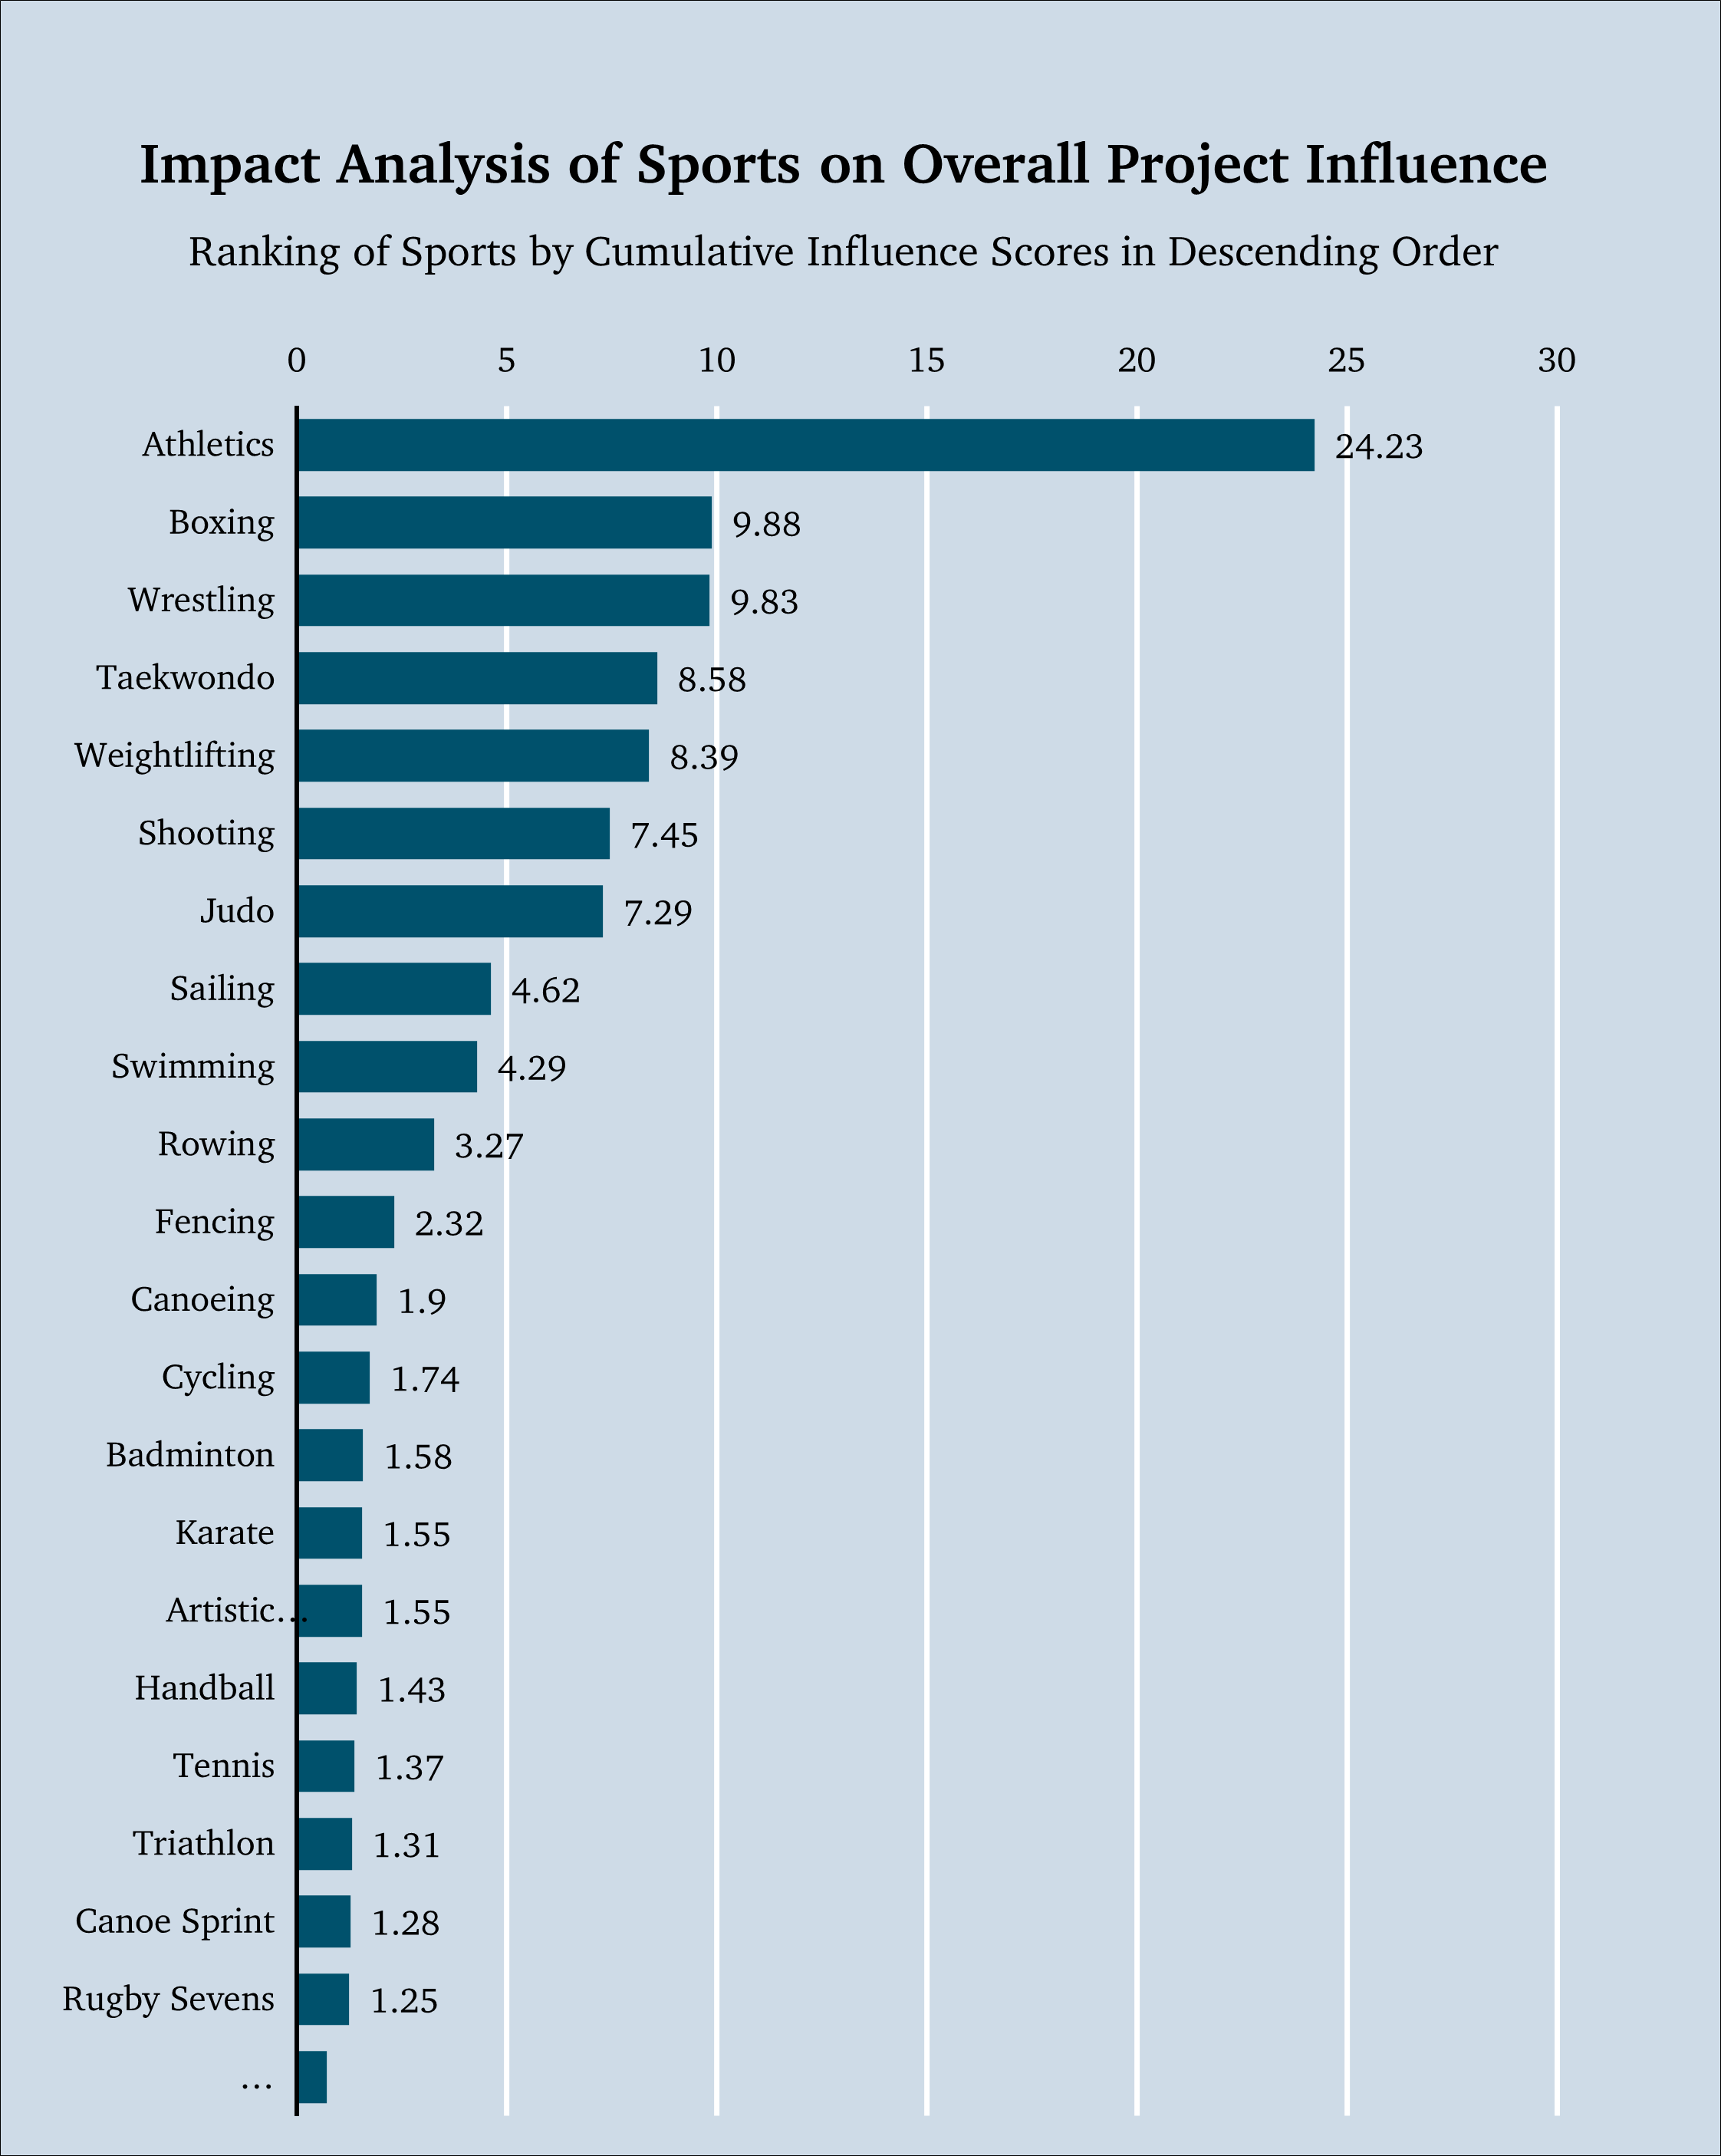
\includegraphics[width=0.9\linewidth,height=10cm]{pics/sport_influence_whole.png}
    \caption{Ranking of sports by global importance based on aggregated event importance values across all countries.}
    \label{fig:sport_importance}
\end{wrapfigure}



\paragraph{Step 4}
The sports are then ranked based on their global importance values $W_k$. A visualization of the rankings illustrates that athletics, boxing, and wrestling are the top three most important sports globally, where athletics has the abosolute highest(more than twice of the second place) importance value.

\subsubsection{Results and Insights}
The analysis reveals that the importance of sports varies significantly across countries. The ranking of sports based on global importance highlights sports such as athletics, swimming, and gymnastics as the most influential globally. These sports typically feature a larger number of events and offer more medal opportunities, which contributes to their higher global importance.

\subsubsection{Discussion and Recommendations}
\begin{itemize}
    \item Countries with limited resources should focus on events with higher importance values $w_{i,j}$ for their specific contexts, as these events offer the best return on investment for medal performance.
    \item Policies that encourage diversification in participation could help countries improve their standings in globally important sports.
    \item Further analysis can include regional comparisons or investigate the temporal trends of sport importance over multiple Olympic cycles.
\end{itemize}


\subsection{Subtask}

\section{Task2 --- The Great Coach Effect: its identification and impact}

The Great Coach Effect is a phenomenon where the presence of a highly skilled coach significantly improves the performance of athletes. Due to the fact that coaches are not bound to a specific country, they can have a significant impact on the medal counts of multiple nations. Identifying the Great Coach Effect and quantifying its impact on medal counts is crucial for predicting Olympic success.

\subsection{Identification}

\subsubsection{Methodology}

We reckon that the Great Coach Effect can be identified by comparing the performance of athletes under the same coach across different countries. It should, by nature, cause one country to have a sharp increase in their medal count in specific sports (otherwise this coach wouldn't be that great), and one other country to go through a gradual-to-sharp decrease in their medal count in the same sports. This is because the coach basically can only focus on coaching one country simultaneously, and the athletes from the other country would not receive the same level of training and support.

Again, due to the inherent limitation of usable dataset, we can only seek to identify the Great Coach Effect from this characteristic, rather than other methods such as relying on coach information to deduce the effect.

Therefore, we propose a two-step approach to identify and quantify the Great Coach Effect:

\begin{enumerate}
    \item Identify such pattern across the dataset.
    \item Refer to outside sources to interpret and cross-verify the result, finding out which specific coach is causing the effect each time.
\end{enumerate}

\subsubsection{Implementation}

We implemented the data filtering logic in Python with 0.23k LOC. The program reads the dataset, groups the data by country, sport, and year, and calculates the weighted medal count for each combination(gold medals with weight 3, silver with 2 and bronze with 1). It then uses linear regression on the most recent 12 years of data to calculate the slope of the medal trend over time. A positive slope exceeding a defined threshold (POS\_K\_LOWER) indicates a sharp increase, while a negative slope below another threshold (NEG\_K\_UPPER) indicates a gradual-to-sharp decrease. Countries with significant trends are recorded as having possible increases or decreases.

The program then pairs countries with overlapping trends in the same sport, checking the overlap period to ensure it spans at least four years and does not exceed a defined gap (OVERLAP\_GAP\_UPPER). Paired trends suggest the transfer of coaching expertise from one country to another.

By carefully calibrating the thresholds and gaps, we can effectively identify the Great Coach Effect and quantify its impact on national performances.

\begin{figure}[htbp]
    \begin{minipage}[t]{0.5\textwidth}
        \centering
        \includegraphics[width=0.8\textwidth]{pics/great_coach_effect_analysis_(sport_level).png}
    \end{minipage}
    \begin{minipage}[t]{0.5\textwidth}
        \centering
        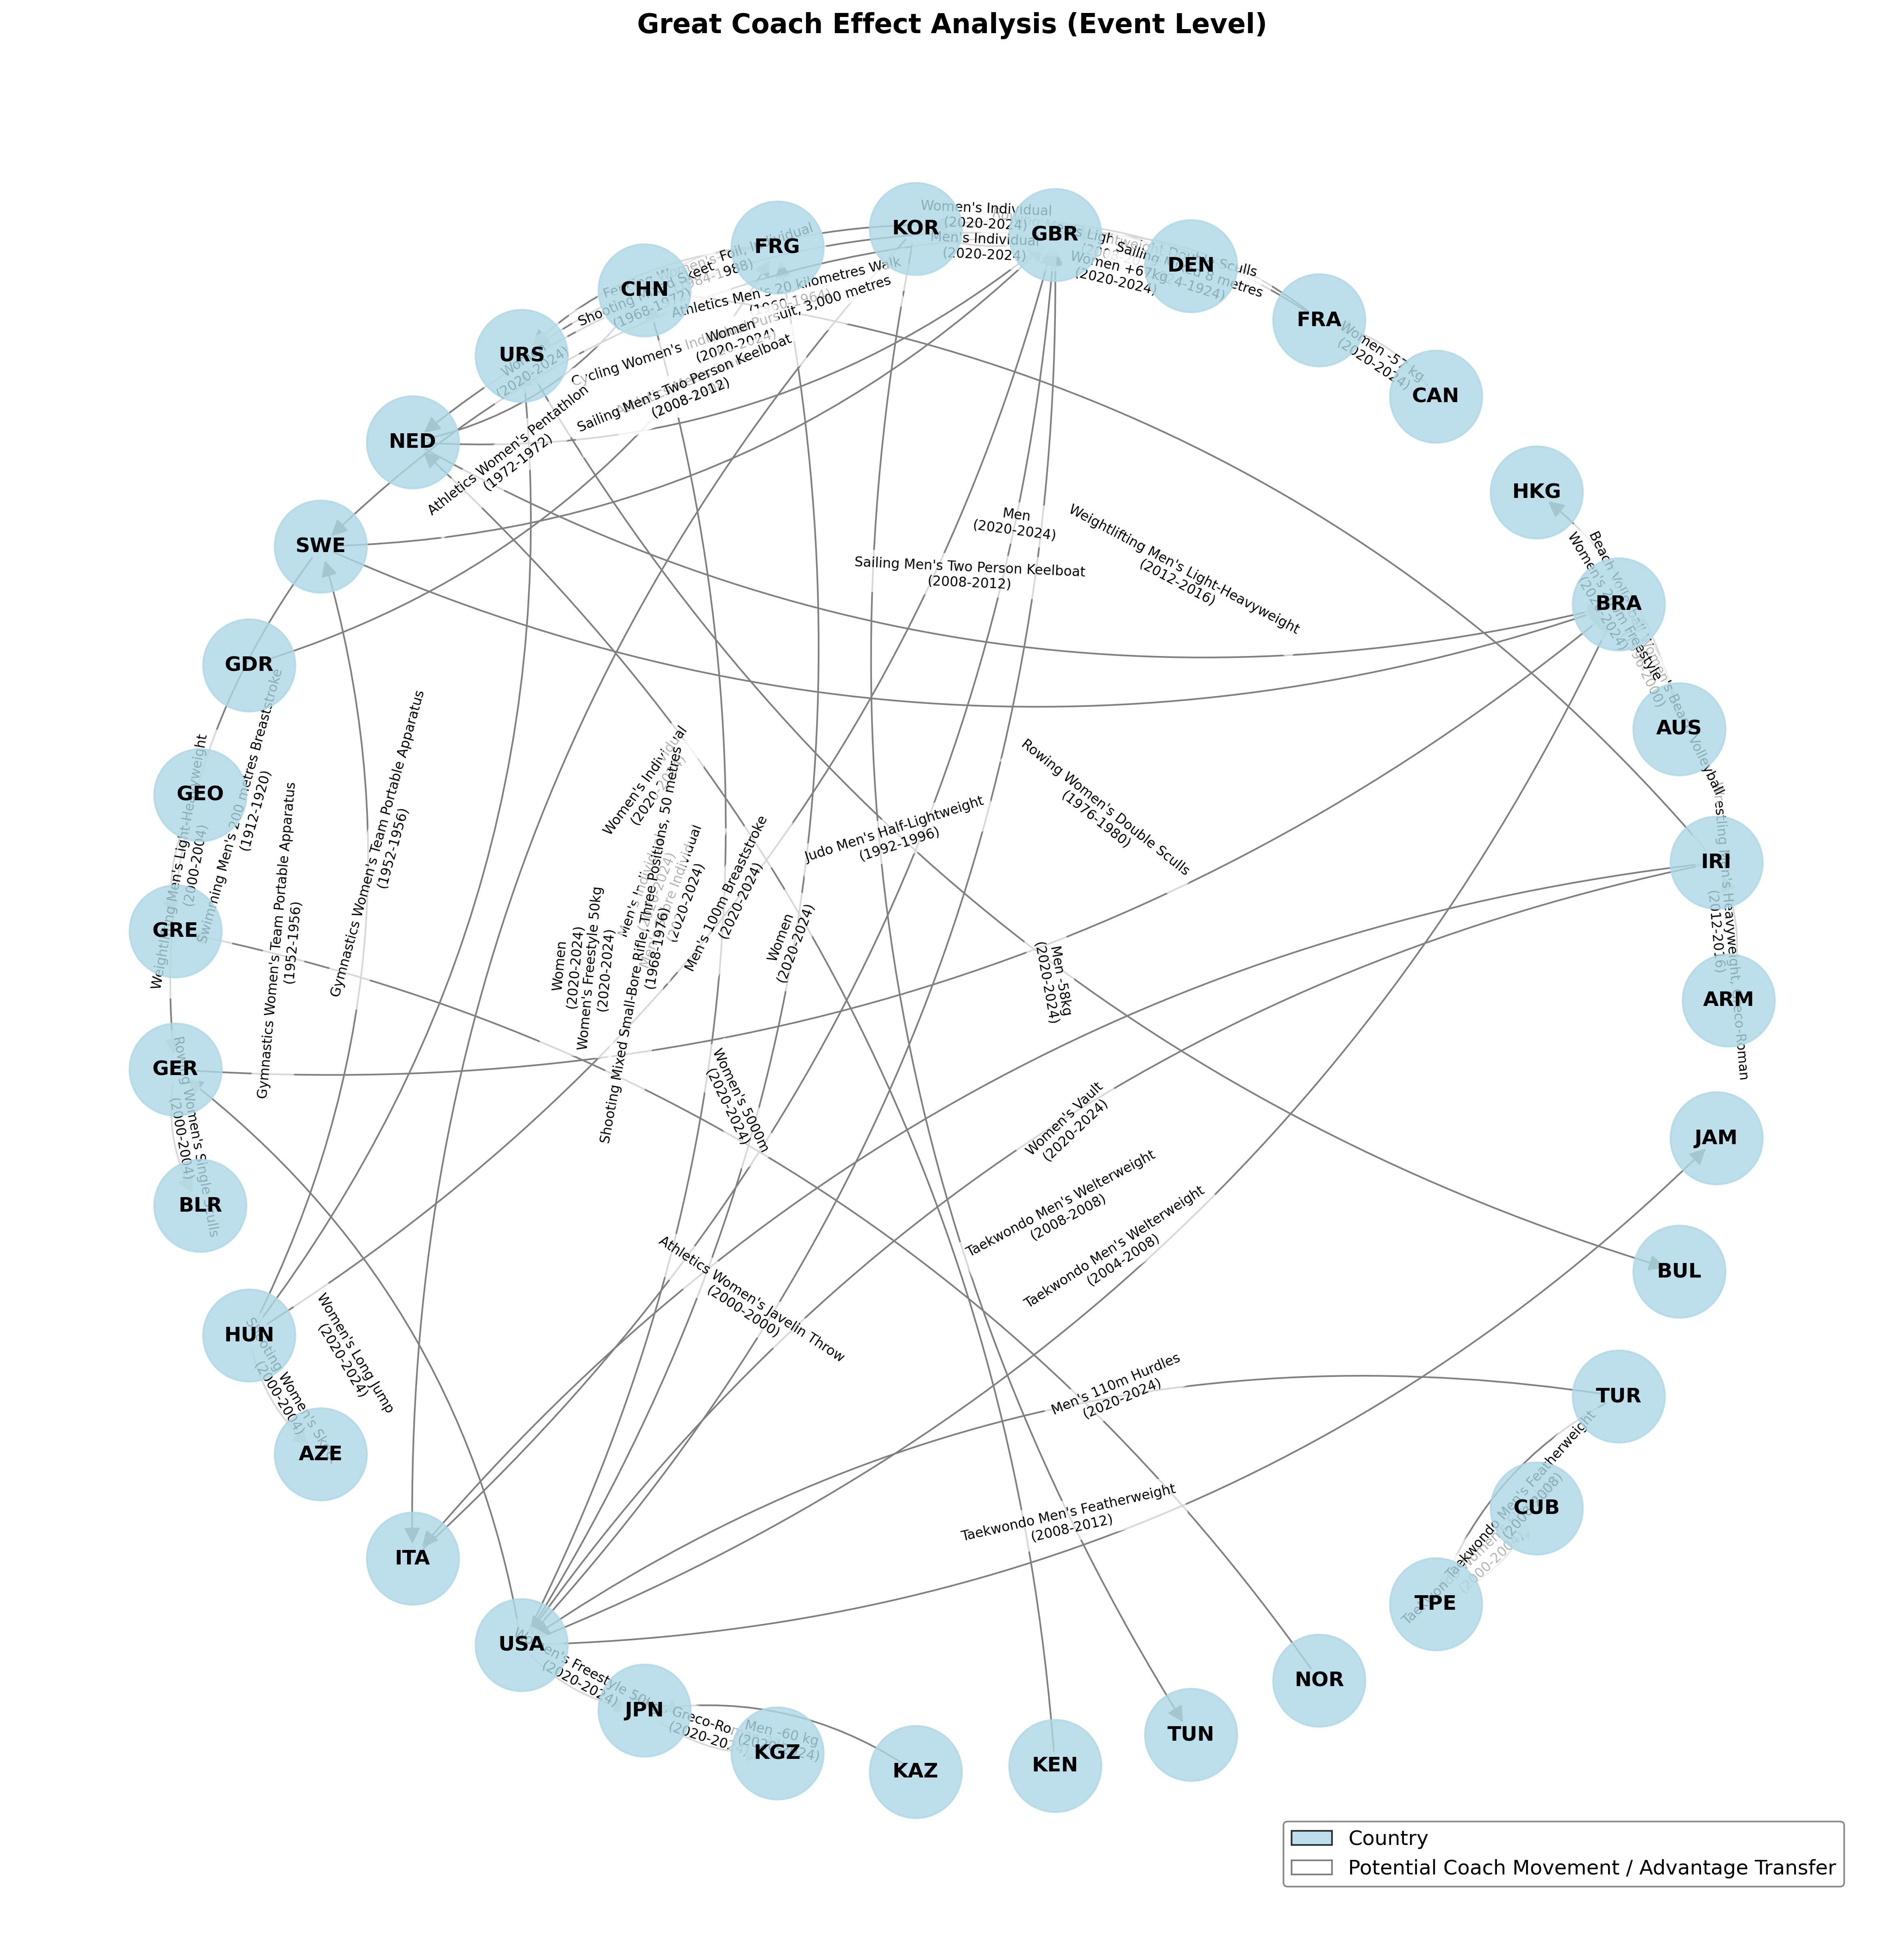
\includegraphics[width=0.8\textwidth]{pics/great_coach_effect_analysis_(event_level).png}
    \end{minipage}
    \caption{Potential occurences of The Great Coach Effects from sport level and event level}
\end{figure}

However elaborate we may calibrate the parameters, there still exists the issue of false positives and false negatives, with false positives accounting more because other factors may also contribute to this same characteristic. We recommend cross-referencing the results with external sources, such as coaching records and athlete interviews, to validate the findings and pinpoint the specific coaches responsible for these shifts. This data-driven approach allows for systematic identification of the Great Coach Effect, providing actionable insights into the strategic importance of coaching in achieving Olympic success.

\subsection{Quantification}

\subsubsection{Methodology}

We will quantify two main aspects of the Great Coach Effect: the magnitude of the performance change in both medal counts changes and the percentage of that change to the total medal count of the country.

The magnitude of the performance change can be calculated by comparing the average medal count before and after the coach transfer, while the percentage of the change can be calculated by dividing the change in medal count by the total medal count of the country in the respective sport.

These two aspects, especially the percentage of medal change to the total medal count of the country, have inextricable correlations with the overall strength of the country. Therefore, we will employ the same strategy as in our model establishment to cluster countries based on their historical medal counts, and then quantify the Great Coach Effect within each cluster.


\subsubsection{Implementation}

We further polish the program used in the identification step to calculate the magnitude and percentage of the Great Coach Effect, adding an additional 0.23k LOC. The program categorizes countries based on their tier value, calculates the average increase/decrease in medal count, and computes the average percentage of this change relative to the total medal count of the country. These metrics provide a comprehensive view of the Great Coach Effect's potential impact on different countries and sports.

\begin{figure}[htbp]
    \centering
    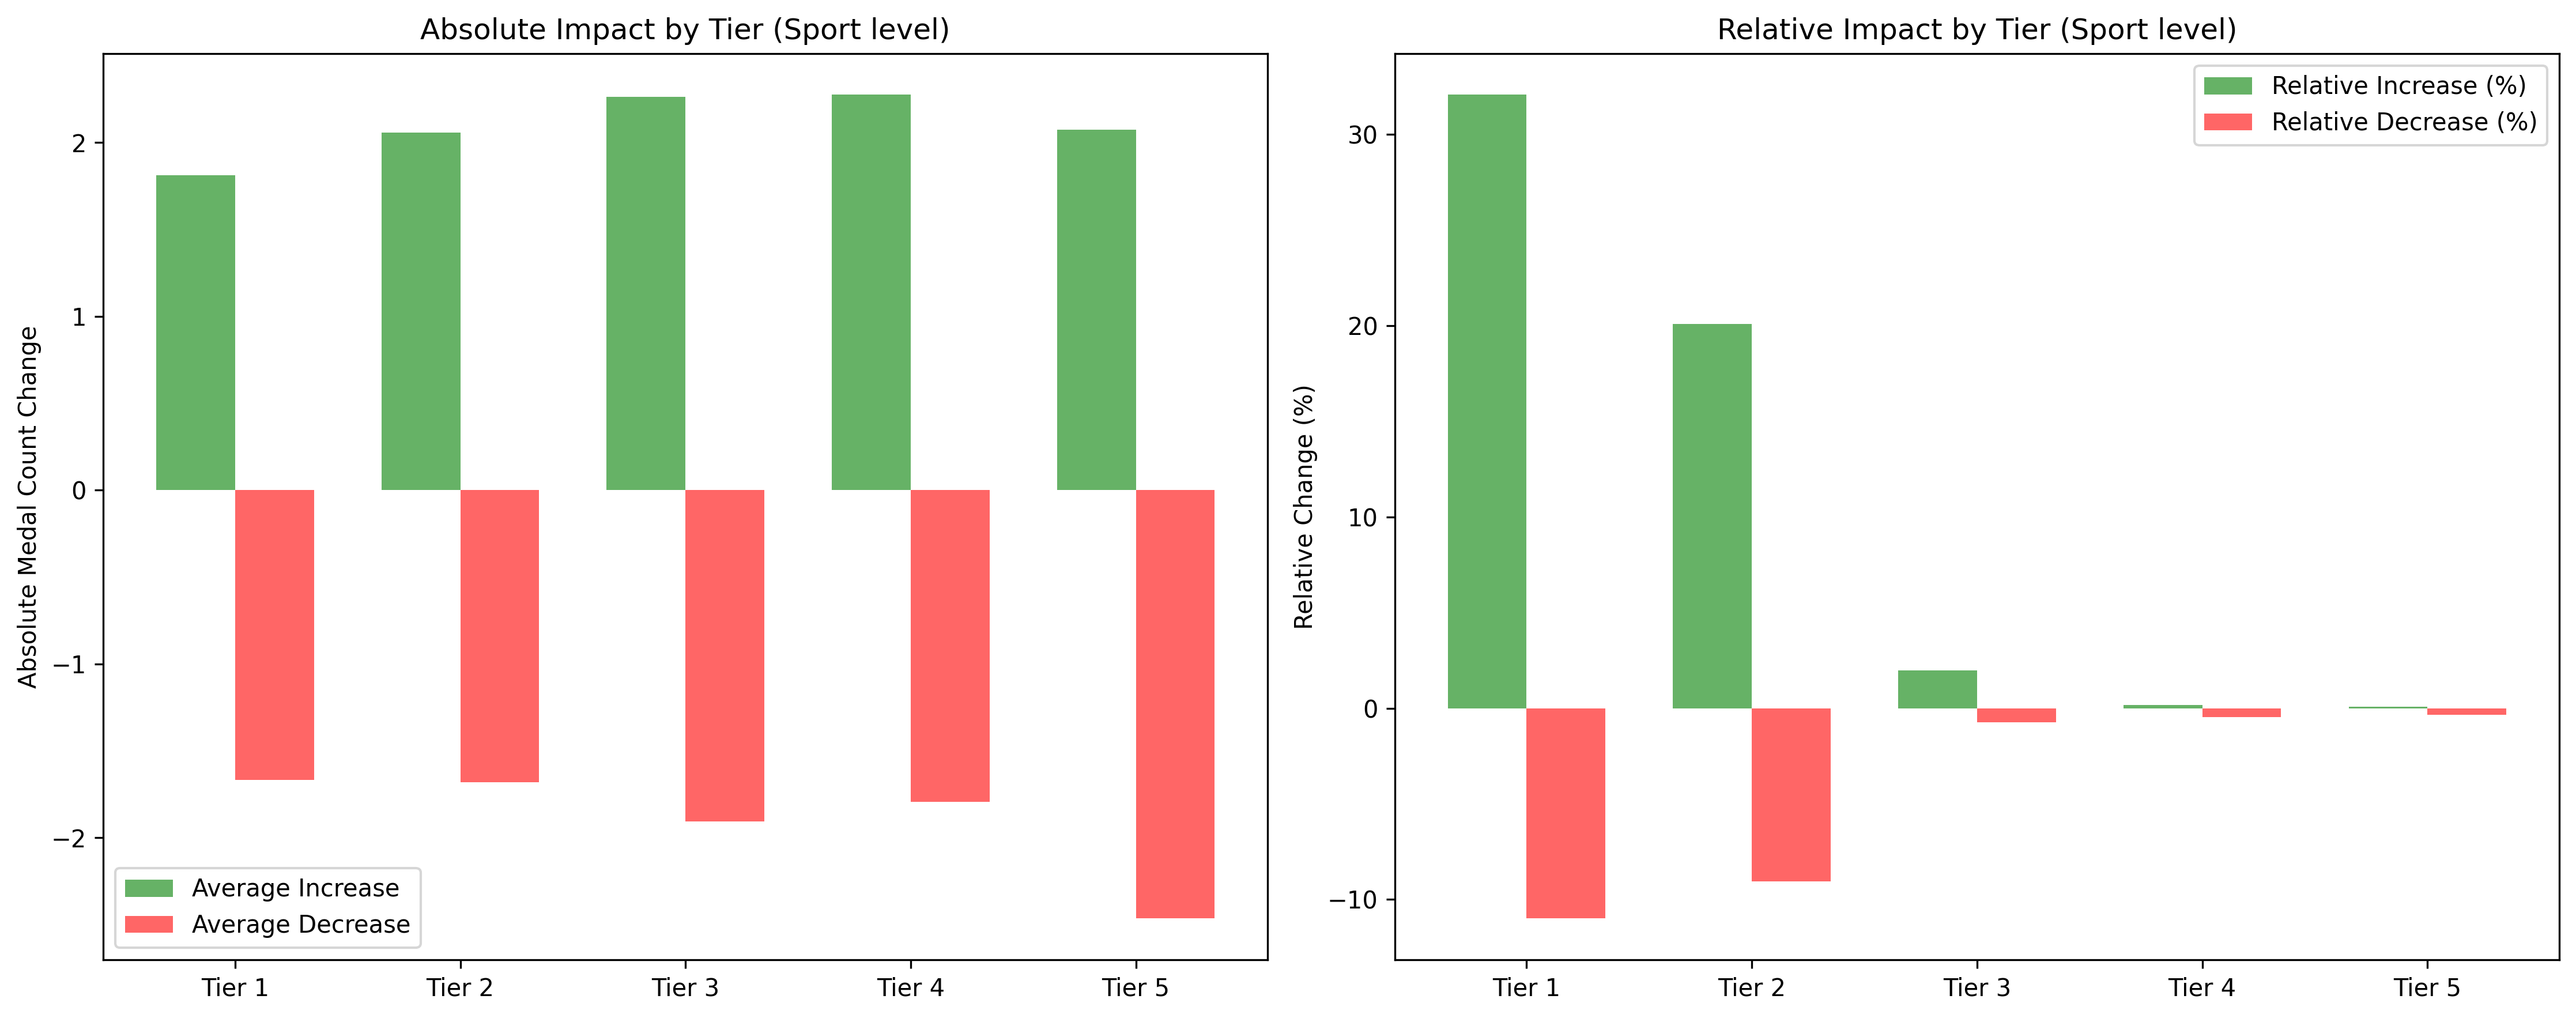
\includegraphics[width=0.8\textwidth]{pics/coach_effect_impact_Sport_from_csv.png}
    \caption{Quantification of The Great Coach Effect}
\end{figure}

\begin{table}[htbp]
    \centering
    \begin{tabular}{|c|c|c|c|c|}
        \hline
        Tier & Avg. Increase & Avg. Decrease & Relative Increase(\%) & Relative Decrease(\%) \\
        \hline
        1 & 1.8125 & -1.6667 & 32.0772 & -10.9944 \\
        \hline
        2 & 2.0562 & -1.6795 & 20.1028 & -9.0563 \\
        \hline
        3 & 2.2623 & -1.9041 & 1.9766 & -0.7317 \\
        \hline
        4 & 2.2743 & -1.7923 & 0.1780 & -0.4518 \\
        \hline
        5 & 2.0746 & -2.4638 & 0.0660 & -0.3472 \\
        \hline
    \end{tabular}
    \caption{Impact of The Great Coach Effect on Different Tiers of Countries}
\end{table}

This figure clearly shows the impact of the Great Coach Effect on different tiers of countries, highlighting the potential for significant performance improvements under the guidance of elite coaches. We can see that the positive and negative impact of the Great Coach Effect(namely, the moving in and out of great coaches) on absolute medal changes has remained constant among different tiers of countries, while its impact on relative medal changes decreases as the tier goes up. This is an expected phenomenon because countries with better overall power already do well in sports across a wide range of fields, so the arrival or departure of one specific coach won't have much effect relative to the total medal count. By quantifying the magnitude and percentage of the effect, we can better understand the strategic value of investing in high-caliber coaching talent and its implications for national Olympic success.

\subsection{Exemplification}
By analyzing the performance trends in specific sports, we identified notable cases where the transfer of a coach coincided with a sharp increase in performance of one country and a decline or stagnation for another, allowing for the cross-verification of our algorithms. Below are three exemplifications of the Great Coach Effect based on historical Olympic data and their correlations with our results.\

It is worth mentioning that the data generated by the program above provides pairs of trends where one country's performance in a certain event increases significantly while another decreases over the same period of time. To spot such pattern, we assign each kind of medal with a value and apply linear regression to the data over a certain of range to get the slope, where a positive slope indicates improvement and vice versa.

\subsubsection{Synchronized Swimming Women's Team: Ana Tarré}
\begin{lstlisting}
- Event: Synchronized Swimming Women's Team, Overlap Years [2008-2012], Increase: CHN(slope=0.125) / Decrease: ESP(slope=-0.250)
\end{lstlisting}

This piece of data generated by the program reveals a significant overlap in performance trends between China (CHN) and Spain (ESP) during the period from 2008 to 2012. China's positive slope (0.125) and Spain's negative slope (-0.250) aligns well with Ana Tarré's transition from coaching Spain to China in 2012.

As we gather the data of a longer period, Ana Tarré's influence as a coach is clearly reflected in the medal trends for synchronized swimming. During her tenure with Spain (1996–2012), the team gradually improved, earning higher medals, peaking with a Silver medal in 2008 and a Bronze in 2012. However, after she transitioned to coaching China in 2012, Spain had dropped out of the podium positions since then until 2024, while China experienced a gradual rise, achieving a series of Silver medals and finnaly a Gold medal in 2024. This shift strongly aligns with the Great Coach Effect, as her expertise and strategies appear to have propelled China's team to the top while Spain struggled without her guidance.

\subsubsection{Gymnastics Women's Team All-Around: Béla Károlyi}
\begin{lstlisting}
- Event: Gymnastics Women's Team All-Around, Overlap Years [2000-2008], Increase: USA(slope=0.125) / Decrease: ROU(slope=-0.250)
\end{lstlisting}

According to the program data, the overlap period between Romania (ROU) and the United States (USA) spans from 2000 to 2008. During this time, Romania exhibited a steep negative slope (-0.250), whereas the United States showed a positive one (0.125), which matches the historical narrative of Béla Károlyi's influence.

Béla Károlyi's legendary coaching career demonstrates a clear pattern of the Great Coach Effect. While coaching Romania (1974–1981), he elevated the team to global prominence, culminating in Silver medals in 1976 and 1980. After moving to coach the United States (1981–2016), Romania's performance declined, while the U.S. women's gymnastics team emerged as a dominant force, securing multiple Gold medals, including in 1996, 2012, and 2016. The sharp contrast in medal trends between the two nations during and after his coaching periods highlights his pivotal role in shaping team success.

\subsubsection{Women's Volleyball: Lang Ping}
\begin{lstlisting}
- Event: Volleyball Women's Volleyball, Overlap Years [1992-2004], Increase: CHN(slope=0.175) / Decrease: USA(slope=-0.075)
- Event: Volleyball Women's Volleyball, Overlap Years [2004-2012], Increase: USA(slope=0.250) / Decrease: CHN(slope=-0.375)
\end{lstlisting}

The program identifies two overlapping periods: 1992-2004 and 2004-2012. In both periods, one of CHN/USA rises and the other falls, which closely corresponds to Lang Ping's coaching career.

Looking at Lang Ping's coaching career spanning over 20 years, we can also discover the distinct influence of a capable coach. During her first tenure with China (1995-2005), the team achieved notable successes, including a Gold medal in 2004. After transitioning to coach the U.S. team (2005-2013) which had won few medals in history, U.S. quickly surpassed China and won 2 consecutive Silver medals. When Lang Ping returned to coach China in 2013, the Chinese team quickly regained its dominance with a Gold in 2016. This fluctuation in performance underscores her unique ability to transform teams and highlights the strategic importance of securing top-tier coaching talent.

% These examples illustrate how the transfer of elite coaches can create significant shifts in medal performance across countries, substantiating the Great Coach Effect. The patterns not only validate the causality between coaching expertise and medal counts but also provide insights for national Olympic committees to consider investing in high-caliber coaching for sustained success.

\subsection{Recommendation}

In the Quantification part, we represented that the Great Coach Effect has a consistent impact on the absolute medal count changes across different tiers of countries, while its impact on relative medal count changes decreases as the tier goes up. This suggests that investing in elite coaching talent can yield substantial performance improvements, particularly for countries with lower historical medal counts(represented by low tier).

Therefore, we recommend that national Olympic committees prioritize recruiting and retaining top-tier coaches for tier 2 countries. Tier 1 countries usually have too tight a budget to afford the cost of coaches with great expertise, while it won't be really necessary for tier 3~5 countries to do so because of the low relative effect.

To determine which three tier 2 countries can benefit the most from the Great Coach Effect, we use the python code from Quantification part and modifies it to find the 3 countries with the highest potential for performance improvement. 

\begin{figure}[htbp]
    \centering
    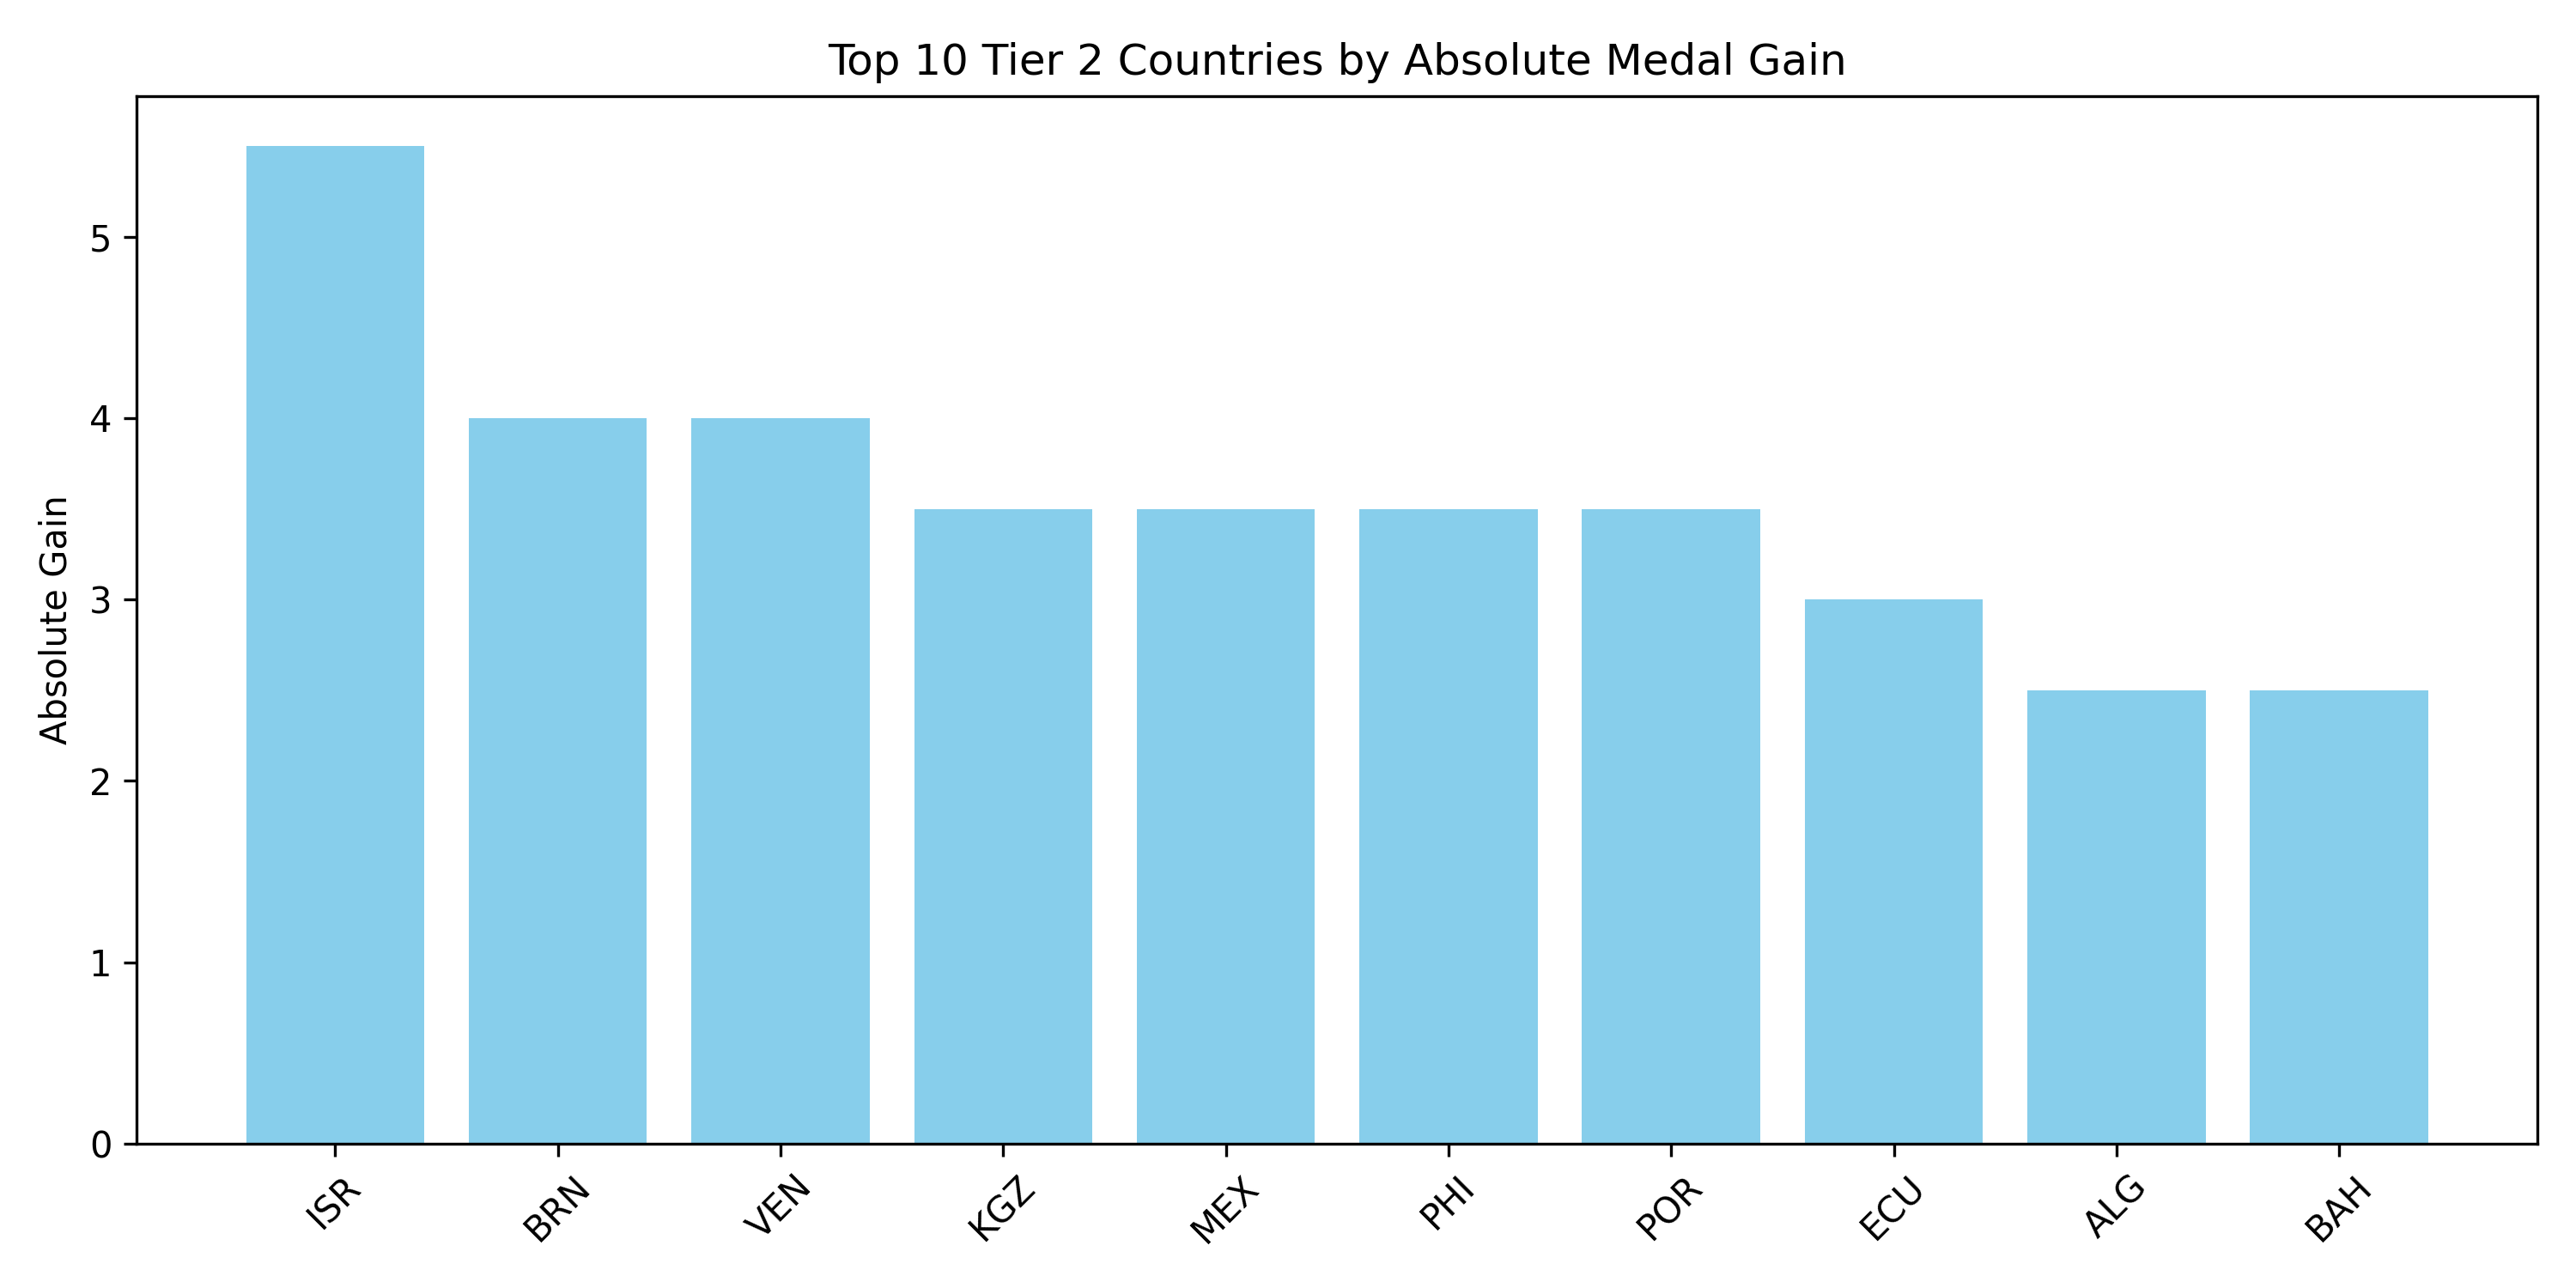
\includegraphics[width=0.8\textwidth]{pics/tier2_top10_absolute_gain.png}
    \caption{Quantification of The Great Coach Effect on Tier 2 Countries}
\end{figure}

From the figure above, we recommend the top 3 countries with the highest potential for performance improvement: ISR (Israel), BRN (Bahrain), and VEN (Venezuela), with respective projected medal gain of 5.5, 3.9 and 3.9.


\section{Task3 --- Original Insights revealed from the model}










\section{Sensitivity Analysis}

\subsection{Strengths}

\subsection{How to cite?}
bibliography cite use \cite{1}

% AI cite use \AIcite{AI1,AI2,AI3}

\begin{thebibliography}{99}
    
    \bibitem{1} Ball, D. W. (1972). Olympic Games competition: Structural correlates of national success. International Journal of Comparative Sociology, 15, 186–200.
    \bibitem{2} Bernard, A. B., \& Busse, M. R. (2004). Who wins the Olympic Games: Economic resources and medal totals. Review of Economics and Statistics, 86, 414–417.
    \bibitem{3} Bian, X. (2005). Predicting Olympic Medal Counts: The Effects of Economic Development on Olympic Performance. The Park Place Economist, 13, 37-44.
    \bibitem{4} Forrest, D., Sanz, I., \& Tena, J. D. (2010). Forecasting national team medal totals at the Summer Olympic Games. International Journal of Forecasting, 26, 576–588.
    \bibitem{5} Schlembach, C., Schmidt, S. L., Schreyer, D., \& Wunderlich, L. (2022). Forecasting the Olympic medal distribution – A socioeconomic machine learning model. Technological Forecasting \& Social Change, 175, 121314.
    \bibitem{6} Tcha, M., \& Pershin, V. (2003). Reconsidering performance at the Summer Olympics and revealed comparative advantage. Journal of Sports Economics, 4, 216–239.
    \bibitem{7} Bernard A B, Busse M R. Who wins the Olympic Games: Economic resources and medal totals[J]. Review of economics and statistics, 2004, 86(1): 413-417.
    \bibitem{8} Xue, J., \& Shen, B. (2020). A novel swarm intelligence optimization approach: sparrow search algorithm. \textit{Systems Science \& Control Engineering, 8}(1), 22-34.
    \bibitem{9} Xue, J., \& Shen, B. (2023). Dung beetle optimizer: A new meta-heuristic algorithm for global optimization. \textit{The Journal of Supercomputing, 79}(7), 7305-7336.
    \bibitem{10} Mirjalili, S. (2016). SCA: a sine cosine algorithm for solving optimization problems. \textit{Knowledge-Based Systems, 96}, 120-133.
    \bibitem{11} Steinbrunn, M., Moerkotte, G., \& Kemper, A. (1997). Heuristic and randomized optimization for the join ordering problem. \textit{The VLDB Journal, 6}, 191-208.
    \bibitem{12} Zhan, Z. H., Zhang, J., Li, Y., \& Chung, H. S. H. (2009). Adaptive particle swarm optimization. \textit{IEEE Transactions on Systems, Man, and Cybernetics, Part B (Cybernetics), 39}(6), 1362-1381.
    \bibitem{13} Hashim, F. A., \& Hussien, A. G. (2022). Snake Optimizer: A novel meta-heuristic optimization algorithm. \textit{Knowledge-Based Systems, 242}, 108320.
    \bibitem{14} Trojovský, P., \& Dehghani, M. (2022). Pelican optimization algorithm: A novel nature-inspired algorithm for engineering applications. \textit{Sensors, 22}(3), 855.
    \bibitem{15} Mirjalili, S., Mirjalili, S. M., \& Lewis, A. (2014). Grey wolf optimizer. \textit{Advances in Engineering Software, 69}, 46-61.
    \bibitem{16} Nadimi-Shahraki, M. H., Taghian, S., \& Mirjalili, S. (2021). An improved grey wolf optimizer for solving engineering problems. \textit{Expert Systems with Applications, 166}, 113917.
    \bibitem{17} Abdollahzadeh, B., Gharehchopogh, F. S., \& Mirjalili, S. (2021). African vultures optimization algorithm: A new nature-inspired metaheuristic algorithm for global optimization problems. \textit{Computers \& Industrial Engineering, 158}, 107408.


\end{thebibliography}

\begin{appendices}

\section{First appendix}

% In addition, your report must include a letter to the Chief Financial Officer (CFO) of the Goodgrant Foundation, Mr. Alpha Chiang, that describes the optimal investment strategy, your modeling approach and major results, and a brief discussion of your proposed concept of a return-on-investment (ROI). This letter should be no more than two pages in length.

\begin{letter}{Dear, Mr. Alpha Chiang}

    \vspace{\parskip}

    Sincerely yours,

    Your friends

\end{letter}

\section{Second appendix}

    % \lstinputlisting[language=C++]{./code/mcmthesis-sudoku.cpp}

\end{appendices}

% AI report begins here
\AImatter
\begin{ReportAiUse}{9}
\bibitem{AI1}



\end{ReportAiUse}

\end{document}
